\documentclass{article}

\usepackage{geometry}

\usepackage{amsmath}
\usepackage{amsfonts}
\usepackage{amssymb}
\usepackage[T1, T2A]{fontenc}
\usepackage[utf8]{inputenc}
\usepackage[english, russian]{babel}
\usepackage{graphics}
\usepackage{amsthm}
\usepackage{hyperref}
\usepackage{fancyhdr}
\usepackage{wrapfig}
\usepackage[dvips]{graphicx}
\graphicspath{{img/}}
\usepackage{float}
\usepackage{datetime}

\hypersetup{
colorlinks,
citecolor=black,
filecolor=black,
linkcolor=black,
urlcolor=black
}

\geometry{
a4paper,
total={170mm,260mm},
left=20mm,
top=20mm,
}

\renewcommand{\v}[1]{{\overline{#1}}}
\newcommand{\norm}[1]{{\parallel #1 \parallel}}
\newcommand{\abs}[1]{{\left| #1 \right|}}
\newcommand{\ea}{\v{e}_1}
\newcommand{\eb}{\v{e}_2}
\newcommand{\ec}{\v{e}_3}
\newcommand{\ei}{\v{e}_i}
\newcommand{\ek}{\v{e}_k}
\newcommand{\el}{\v{e}_l}
\newcommand{\re}[1]{(\ref{#1})}
\newcommand{\R}{\mathbb{R}}
\newcommand{\pd}[2]{\frac{\partial #1}{\partial #2}}
\newcommand{\pdd}[2]{\frac{\partial}{\partial #2} \left(#1\right)}

\newcounter{lecturesCounter}
\newcommand{\lline}[1]{\subsection*{
\centering\stepcounter{lecturesCounter}\underline{Лекция \arabic{lecturesCounter} от #1}}}

\allowdisplaybreaks

\DeclareMathOperator{\grad}{grad}
\DeclareMathOperator{\rot}{rot}
\DeclareMathOperator{\rank}{rank}
\DeclareMathOperator{\diag}{diag}
% \DeclareMathOperator{\tg}{tg}

\newtheorem*{df}{Определение}
\newtheorem{teo}{Теорема}
\newtheorem{lem}{Лемма}
\newtheorem{prp}{Предложение}
\newtheorem{hyp}{Предположение}
\newtheorem{ass}{Утверждение}
\newtheorem*{cor}{Следствие}
\newtheorem*{ntc}{Замечание}
\newtheorem*{xmp}{Пример}

\renewcommand\qedsymbol{$\blacksquare$}

\newcommand{\lb}{\left(}
\newcommand{\rb}{\right)}


% \setcounter{secnumdepth}{0}
\setcounter{tocdepth}{2}

\newdate{date}{09}{02}{2018}
\date{\displaydate{date}}

\author{Муницына Мария Александровна}
\title{Лекции по аналитической механике. Осенний семестр.}

\begin{document}
  \label{title}
  \vfill
  \begin{titlepage}
  
  \maketitle
  \begin{center}
  {\itshape\small Набор и рисунки: Александр Валентинов.\\
    За рукописные конспекты спасибо Павлу Цаю и Никите Свешникову.}
  \vspace{1em}

  {\itshape\small Исходный код: \url{https://github.com/valentiay/analmech}}
  \vspace{5em}

  \fbox{\begin{minipage}{25em}
    \centering
    Конспект не проходил проффесиональную редактуру и может содержать смысловые ошибки
  \end{minipage}}
  \vfill

  \end{center}
  \thispagestyle{empty}
  \end{titlepage}

  \pagestyle{fancy}
  \renewcommand{\footrulewidth}{0.2mm}
  \fancyhead{}
  % \fancyhead[L,R]{}
  \fancyhead[L]{\hyperref[title]{М.А. Муницына}} 
  \fancyhead[R]{\hyperref[title]{Лекции по аналитической механике. Осенний семестр.}} 
  \fancyfoot[C]{\thepage}
  
  \pagebreak
  \tableofcontents
  \pagebreak
  
  \lline{06.09.2017}  \section{Кинематика точки}
  \begin{df}
  Материальная точка - точка, размером которой можно пренебречь.
  \end{df}
  
  \noindent Мы будем полагать, что время меняется равномерно и непрерывно.
  \begin{center}  
  \begin{picture}(100, 100)
  \put(40,40){\vector(1,0){50}} %
  \put(40,40){\vector(0,1){50}} %
  \put(40,40){\vector(-1, -1){25}} %
  \put(40,40){\vector(2,1){40}} %
  \put(92,42){$x$} %
  \put(42,92){$z$} %
  \put(8,8){$y$} %
  \put(82,62){$\v{r}$} %
  \qbezier(50,70)(60,80)(80,60) %
  \qbezier(80,60)(85,50)(90,50) %
  \end{picture}
  \end{center}
  \subsection{Векторное описание движения}
  Зависимость координат от времени назовем законом движения.
  $$ \v{r} = \v{r}(t) \in C^2 $$
  \begin{df}
  $ \gamma = \{ \v{r}(t),~ t \in (0,~ +\infty) \} $ - траектория
  \end{df}
  $$ \v{v} = \frac{d\v{r}}{dt} $$
  $$ \v{w} = \frac{d\v{v}}{dt} = \frac{d^2\v{r}}{dt^2} $$
  \subsection{Декартовы координаты}
  $$ \v{r}(t) = x(t)\v{e_x} + y(t)\v{e_y} + z(t)\v{e_z} $$
  $$ \v{v}(t) = \dot x(t)\v{e_x} + \dot y(t)\v{e_y} + \dot z(t)\v{e_z} $$
  $$ \v{w}(t) = \ddot x(t)\v{e_x} + \ddot y(t)\v{e_y} + \ddot z(t)\v{e_z} $$
  \subsection{Движение по окружности}
  $$ 
  \begin{cases}
   x = R \cos \varphi \\
   y = R \sin \varphi
  \end{cases} 
  $$

  $$ 
  \begin{cases}
  \dot x = -R \sin \varphi \cdot \dot \varphi \\
  \dot y = R \cos \varphi \cdot \dot \varphi 
  \end{cases}
  $$
  
  $$ 
  \begin{cases}
  \ddot x = -R \cos \varphi \cdot  \dot \varphi^2 - R \sin \varphi \cdot \ddot \varphi \\
  \ddot y = -R \sin \varphi \cdot  \dot \varphi^2 + R \cos \varphi \cdot \ddot \varphi 
  \end{cases}
  $$
  
  \begin{center}
  \begin{picture}(100,100)
  \put(50,50){\circle{50}} %
  \put(50,50){\line(1,1){14}} %
  \put(50,50){\line(-1,-1){14}} %
  \put(5,50){\vector(1,0){90}} %
  \put(97,52){$x$} %
  \put(50,5){\vector(0,1){90}} %
  \put(52,97){$y$} %
  \put(65,65){$\varphi(t)$} %
  \put(36,36){\vector(1,-1){10}} %
  \put(40,15){$\v{\tau}$} %
  \put(36,36){\vector(1,1){10}} %
  \put(31,40){$\v{n}$} %
  \end{picture}
  \end{center}
  
  $$ \v{v} = R\dot\varphi(-\sin \varphi \cdot \v{e_x} + \cos \varphi \cdot\v{e_y}) = R \dot\varphi \v{\tau} $$
  $$ \v{w} = R \ddot\varphi ( - \sin \varphi \cdot \v{e_x} + \cos \varphi \cdot \v{e_y}) + R \dot\varphi^2(-\cos \varphi \cdot \v{e_x} - \sin \varphi \cdot {\v{e_y}}) = R \ddot \varphi \v{\tau} + R \dot \varphi^2 \v{n}  $$
  
  $$ \v{v} = R \dot\varphi \v{\tau} = v \v{\tau}$$
  $$ \v{w} = R \ddot\varphi \v{\tau} + R \dot \varphi^2 \v{n} = \dot v \v{\tau} + \frac{v^2}{R} \v{n}$$
  
  \subsection{Естественное описание движения}
  Кривая задана параметрически естественным параметром $s$. $ ds = |\v{dr}| \neq 0 $
  \begin{df}
  \begin{equation} 
  \label{tang}
  \v{\tau} = \frac{d\v{r}}{ds} = \vec r' \text{ - касательный вектор}
  \end{equation}
  \begin{equation}
  \label{normal}
  \v{n} = \frac{\vec \tau'}{|\vec {\tau}'|} \text{ - вектор главной нормали }
  \end{equation}
  \begin{equation}    
  \v{b} = [\v{\tau}; \v{n}] \text{ - вектор бинормали }
  \end{equation}  
  \end{df}
  
  \begin{ass} 
  $ \{\v{\tau}, \v{n}, \v{b}\} $ - тройка ортогональных единичных векторов.
  \end{ass}
  \begin{proof}  
  \begin{flalign*}
  & |\v{\tau}| = \frac{|d\v{r}|}{|ds|} = 1 &\\
  & |\v{n}| = \frac{|\v \tau'|}{|\v{\tau}'|} = 1 &\\
  & |\v{\tau}| = 1 \Rightarrow (\tau, \tau) = 1 &\\
  & (\vec {\tau}', \v{\tau}) + (\v{\tau}, \vec {\tau}') = 0 &\\
  & 2 (\v{\tau}', \v{\tau}) = 0 \Rightarrow \v{\tau}' \perp \v{\tau} \Rightarrow \v{n} \perp \v{\tau} &\\
  \end{flalign*}
  
  \end{proof}
  Этот трехгранник называют репер Френе. (Дарбу, сопровождающий трехгранник).
  
  \begin{teo} 
  $ \v{v} = v \v{\tau} $, $ \v{w} = \dot v \v{\tau} + \frac{v^2}{\rho} \v{n} $, где $ v = \dot s $.
  \end{teo}
  \begin{proof}
  \begin{flalign*}
  & \v{v} = \frac{d\v{r}}{dt} = \frac{d\v{r}}{ds} \frac{ds}{dt} = v\v{\tau} &\\
  & \dot{\vec {\tau}} = \frac{d\v{\tau}}{ds} \frac{ds}{dt} = \v{n}kv \text{, по формуле (\ref{normal})} &\\
  & \v{w} = \dot{\vec {v}} = \dot v \v{\tau} + v \dot{\vec {\tau}} = \dot v \v{\tau} + v^2 k \v{n} = \dot v \v{\tau} + \frac{v^2}{\rho} \v{n} &\\ 
  \end{flalign*}
  \begin{flalign*}
  & \dot v \v{\tau} \text{ - касательное ускорение} &\\
  & \frac{v^2}{\rho} \v{n} \text{ - нормальное ускорение } &\\
  & \rho = \frac{1}{|\v r''|} \text{ - радиус кривизны} &\\
  & k = | \v{r}'' | \text{ - кривизна} &\\
  & \v{r}'' \text{ - вектор кривизны} &\\
  \end{flalign*}
  \end{proof}
  
  \paragraph{Формулы Френе:}
  $$ 
  \begin{cases}
  \v{\tau}' = k \v{n} \\
  \v{n}' = - k\v{\tau} + \varkappa \v{b} \\
  \v{b}' = -\varkappa\v{n}
  \end{cases}
  $$
  где $\varkappa$ - коэффициент кручения.
  
  \begin{proof}
  $$ | \v{n} | = 1 \Rightarrow (\v{n}, \v{n}') = 0 $$
  $$ \v{n} \perp \v{\tau} \Rightarrow (\v{n}', \v{\tau}) + (\v{n}, \v{\tau}') = 0 \Rightarrow (\v{n}', \v{\tau}) + k = 0 $$
  
  $$ \v{b}' = [\v{ \tau}', \v{n}] + [\v{\tau}, \v{n}'] = [k\v{n}, \v{n}] + [\v{\tau}, -k\v{\tau} + \varkappa \v{b}] = 0 + \varkappa[\v{\tau}, \v{b}] = -\varkappa\v{n} $$
  \end{proof}
  \subsection{Ортогональные криволинейные координаты}
  
  \begin{figure}[h]
  \centering
  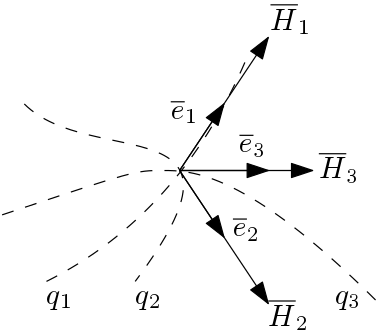
\includegraphics[width=5cm]{fig1.png} 
  \end{figure}  
  
  \begin{gather*}
  \v{r} = \v{r}(q_1(t), q_2(t), q_3(t)) \\
  \v{v} = \dot{\vec {r}}= \sum \limits_{i = 1}^3 \frac{\partial\v{r}}{\partial q_i} \dot q_i\\
  \v{H_i} = \frac{\partial\v{r}}{\partial q_i} = H_i \v{e_i} \text{, где $H_i$ - коэффициенты Ламе.} \\ 
  \end{gather*}
  \subsubsection*{Геометрический смысл}
  $$ ds_i = H_i dq_i $$
  $s_i$ - длина дуги $i$-й координатной линии.
  $$ H_i = \abs{\frac{\partial \v{r}}{\partial q_i}}  = \sqrt{\left(\frac{\partial x}{\partial q_i}\right) ^2 + \left(\frac{\partial y}{\partial q_i}\right) ^2 + \left(\frac{\partial z}{\partial q_i}\right) ^2} $$
  $$ \v{v} = \sum\limits_{i=1}^3 H_i \dot{q_i} \v{e_i},~~ v^2 = (\v{v}, \v{v}) = \sum H_i^2\dot{q_i^2} $$ 
  \begin{teo}
  Компоненты вектора ускорения в ортогональном криволинейном базисе определяются равенством:
  $$ w_i = \frac{1}{H_i}\left(\frac{d}{dt} \frac{\partial}{\partial \dot q_i} \left(\frac{v^2}{2}\right) - \frac{\partial}{\partial q_i} \left(\frac{v^2}{2} \right) \right) $$
  \end{teo}
  \begin{proof}
  \begin{gather*}
(\v{w}, \v{H_i}) = \left(\frac{d\v{v}}{dt}, \frac{\partial \v{r}}{\partial q_i} \right) = \frac{d}{dt} \left(\v{v}, \frac{\partial \v{r}}{\partial q_i}\right) - \left(\v{v}, \frac{d}{dt} \frac{\partial \v{r}}{\partial q_i} \right) \triangleq \\
1) ~ \frac{\partial \v{r}}{\partial q_i} = \frac{\partial \v{v}}{\partial \dot q_i} \text{ - из определения скорости} \\
2) ~ \frac{d}{dt} \left(\frac{\partial \v{r}}{\partial q_i} \right) = \sum \limits_{j = 1}^3 \frac{\partial^2 \v{r}}{\partial q_j \partial q_i} \dot q_j = \sum \limits_{j = 1}^3 \frac{\partial^2 \v{r}}{\partial q_i \partial q_j} \dot q_j = \\ 
= \frac{\partial}{\partial q_i} \left( \frac{d\v{r}}{dt} \right) = \frac{\partial \dot{\vec r}}{\partial q_i} = \frac{\partial \v{v}}{\partial q_i} \\
\triangleq \frac{d}{dt} \left(\v{v}, \frac{\partial \v{v}}{\partial \dot q_i} \right) - \left( \v{v}, \frac{\partial \v{v}}{\partial q_i} \right) = \frac{d}{dt} \frac{1}{2} \frac{\partial}{\partial \dot q_i} (\v{v}, \v{v}) - \frac{1}{2} \frac{\partial}{\partial q_i} (\v{v}, \v{v}) = \\ 
= \frac{d}{dt} \frac{\partial}{\partial \dot q_i} \left(\frac{v^2}{2} \right) - \frac{\partial}{\partial q_i} \left(\frac{v^2}{2}\right) \\
w_i = (\v{w}, \v{e_i}) = \frac{1}{H_i}(\v{w}, \v{H_i})
  \end{gather*}
  \end{proof}
  \lline{13.09.2017}  %2017-09-13
  
  \section{Кинематика твердого тела}
  \begin{df}
  Абсолютно твердым телом называется множество точек, расстояние между которыми не меняется со временем.
  
  $  \{ \v{r_i}, i = \overline{1 \ldots n} ~~:~~|\v{r_i} - \v{r_j} | = C_{ij} = const ,~~ n \geqslant 3 \}$ 
  
  \end{df}

  \begin{figure}[h]
  \centering
  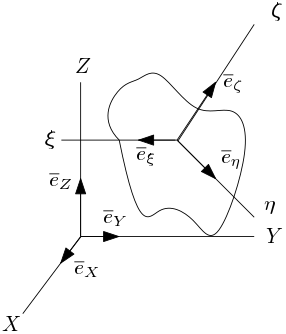
\includegraphics[width=5cm]{fig2.png} 
  \end{figure}  
  $OXYZ$ - неподвижная система отсчета.
  
  $S\xi\eta\zeta$ - связаны с телом (движется).
 
  $$
  X = 
  \left(
  \begin{matrix} 
  (\v{e_{\xi}}, \v{e_{x}}) & 
  (\v{e_{\xi}}, \v{e_{y}}) & 
  (\v{e_{\xi}}, \v{e_{z}}) \\ 
  (\v{e_{\eta}}, \v{e_{x}}) & 
  (\v{e_{\eta}}, \v{e_{y}}) & 
  (\v{e_{\eta}}, \v{e_{z}}) \\  
  (\v{e_{\zeta}}, \v{e_{x}}) & 
  (\v{e_{\zeta}}, \v{e_{y}}) & 
  (\v{e_{\zeta}}, \v{e_{z}}) \\
  \end{matrix}
  \right)
  \text{ - матрица направляющих косинусов.}
  $$
 
  $$ \v{AB} = x\v{e_x} + y\v{e_y} + z\v{e_z} $$
  $$ \v{AB} = \xi\v{e_{\xi}} + \eta\v{e_{\eta}} + \zeta\v{e_{\zeta}} $$

  $$ X
  \left(
  \begin{matrix}
    x \\ y \\ z \\
  \end{matrix}
  \right)
  =
  \left(
  \begin{matrix}
  (\v{e_{\xi}}, x\v{e_x} + y \v{e_y} + z \v{e_z}) \\
  (\v{e_{\eta}}, x\v{e_x} + y \v{e_y} + z \v{e_z}) \\
  (\v{e_{\zeta}}, x\v{e_x} + y \v{e_y} + z \v{e_z}) \\
  \end{matrix}
  \right)
  = 
  \left(
  \begin{matrix}
  (\v{e_{\xi}}, \v{AB}) \\
  (\v{e_{\eta}}, \v{AB}) \\
  (\v{e_{\zeta}}, \v{AB}) \\
  \end{matrix}
  \right)
  =
  \left(
  \begin{matrix}
  \xi \\
  \eta \\
  \zeta \\
  \end{matrix}
  \right)
  =
  \v{\rho}
  $$

  $$ \v{\rho} = X \v{r} $$
  
  \begin{ass}
  $X$ - ортогональная матрица.
  \end{ass}
  \begin{proof}
  $$ XX^T = X^TX = 
  \left(
  \begin{matrix}
  (\v{e_{\xi}}, \v{e_\xi}) & 
  (\v{e_{\xi}}, \v{e_\eta}) & 
  (\v{e_{\xi}}, \v{e_\zeta}) \\
  \vdots & \ddots & \vdots \\
   & \ldots &
  \end{matrix} 
  \right)
  = E $$
  Т.к. базис ортогональный.
  \end{proof} 
  
  $$
  \left(
  \begin{matrix}
  \v{e_{\xi}} \\
  \v{e_{\eta}} \\
  \v{e_{\zeta}} \\
  \end{matrix}
  \right)  
  =  
  X
  \left(
  \begin{matrix}
  \v{e_{x}} \\
  \v{e_{y}} \\
  \v{e_{z}} \\
  \end{matrix}
  \right)
  $$

  $$
  \left(
  \begin{matrix}
  \dot{\v{e_{\xi}}} \\
  \dot{\v{e_{\eta}}} \\
  \dot{\v{e_{\zeta}}} \\  
  \end{matrix}
  \right)
  = 
  \dot{X}
  \left(
  \begin{matrix}
  \v{e_{x}} \\
  \v{e_{y}} \\
  \v{e_{z}} \\
  \end{matrix}
  \right) =
  \underbrace{
  \dot{X} X^T
  }_{\Omega}
  \left(
  \begin{matrix}
  \v{e_{\xi}} \\
  \v{e_{\eta}} \\
  \v{e_{\zeta}} \\
  \end{matrix}
  \right)
  =
  \Omega
  \left(
  \begin{matrix}
  \v{e_{\xi}} \\
  \v{e_{\eta}} \\
  \v{e_{\zeta}} \\
  \end{matrix}
  \right) 
  $$

  $$ \Omega = \dot X X^T $$

  
  \begin{ass}
  $\Omega$ - кососимметрична.
  \end{ass}
  \begin{proof}
  $$ \Omega - \Omega^T = \dot X X^T + (\dot X X^T)^T = \dot X X^T + X \dot {X^T} = \frac{d}{dt}(XX^T) = 
  \frac{d}{dt}(E) = 0 $$
  \end{proof}
  
  \begin{cor}
  $$ \Omega =
  \left(
  \begin{matrix}
  0 & \omega_{\zeta} & -\omega_{\eta} \\
  -\omega_{\zeta} & 0 & \omega_{\xi} \\
  \omega_{\eta} & -\omega_{\xi} & 0 \\
  \end{matrix}
  \right)
  $$
  \end{cor}
  \begin{df}
  $ \v{\omega} = \omega_{\xi}\v{e_{\xi}} + \omega_{\eta}\v{e_{\eta}} + \omega_{\zeta}\v{e_{\zeta}} $ - угловая скорость подвижного репера.
  \end{df}
  
  \subsection{Формулы Пуассона}
  \begin{ass}
  $$ \dot{\v{e_i}} = [\v{\omega}, \v{e_i}],~~ i = \overline{1 \ldots 3} $$
  \end{ass}
  \begin{proof}
  $$
  \dot{\v{e_{\xi}}} = \omega_{\zeta} \v{e_{\eta}} - \omega_{\eta} \v{e_{\zeta}} =
  \begin{vmatrix}
  \v{e_{\xi}} & \v{e_{\eta}} & \v{e_{\zeta}} \\
  \omega_{\xi} & \omega_{\eta} & \omega_{\zeta} \\
  1 & 0 & 0 \\ 
  \end{vmatrix}
  =
  [\v{\omega}, \v{e_{\xi}}] 
  $$
  \end{proof}
  
  \begin{ass}
  $ \v{\omega} = \v{e_{\xi}}(\dot{\v{e_{\eta}}}, \v{e_{\zeta}}) + \v{e_{\eta}}(\dot{\v{e_{\zeta}}}, \v{e_{\xi}}) + \v{e_{\zeta}}(\dot{\v{e_{\xi}}}, \v{e_{\eta}}) $
  \end{ass}
  \begin{proof}
  $$ (\dot{\v{e_{\xi}}}, \v{e_{\eta}}) = \omega_{\zeta} $$
  $$ (\dot{\v{e_{\eta}}}, \v{e_{\zeta}}) = \omega_{\xi} $$
  $$ (\dot{\v{e_{\zeta}}}, \v{e_{\xi}}) = \omega_{\eta} $$
  \end{proof}
  
  \begin{ass}
  $ \v{\omega} = \frac{1}{2} ([\v{e_{\xi}}, \dot{\v{e_{\xi}}}] + [\v{e_{\eta}}, \dot{\v{e_{\eta}}}] + [\v{e_{\zeta}}, \dot{\v{e_{\zeta}}}]) $
  \end{ass}
  \begin{proof}
  $$ \v{\omega} 
  = \frac{1}{2} ([\v{e_{\xi}}, \dot{\v{e_{\xi}}}] + [\v{e_{\eta}}, \dot{\v{e_{\eta}}}] + [\v{e_{\zeta}}, \dot{\v{e_{\zeta}}}]) 
  = \frac{1}{2} ([\v{e_{\xi}}, [\v{\omega}, \v{e_{\xi}}]] + [\v{e_{\eta}}, [\v{\omega}, \v{e_{\eta}}]] + [\v{e_{\zeta}}, [\v{\omega}, \v{e_{\zeta}}]]) = $$
  $$ = \frac{1}{2} \left( \v{\omega}(\v{e_{\xi}}, \v{e_{\xi}}) - \v{e_{\xi}}(\v{\omega}, \v{e_{\xi}}) + \v{\omega}(\v{e_{\eta}}, \v{e_{\eta}}) - \v{e_{\eta}}(\v{\omega}, \v{e_{\eta}}) + \v{\omega}(\v{e_{\zeta}}, \v{e_{\zeta}}) - \v{e_{\zeta}}(\v{\omega}, \v{e_{\zeta}}) \right) = $$ 
  $$ = \frac{1}{2}(3\v{\omega} - \v{\omega}) = \v{\omega} $$
  \end{proof}
  
  \begin{xmp}
  Угловая скорость репера Френе.
  $$ 
  \begin{cases}
  \v{\tau}' = k \v{n} \\
  \v{n}' = - k\v{\tau} + \varkappa \v{b} \\
  \v{b}' = -\varkappa\v{n}
  \end{cases}
  $$
  
  $$
  \begin{cases}
  \dot{\v{\tau}} = \frac{d\v{\tau}}{ds} \dot s \\
  \dot{\v{n}} = \frac{d\v{n}}{ds} \dot s \\
  \dot{\v{b}} = \frac{d\v{b}}{ds} \dot s \\
  \end{cases} 
  $$
  
  $$ \v{\omega} = \v{\tau}(\dot s (-k\v{\tau} + \varkappa\v{b}), \v{b}) + \v{n}(\dot s (-\varkappa\v{n}, \v{\tau}) + \v{b}(\dot s(k \v{n}), \v{n}) = \dot s (\varkappa\v{\tau} + k\v{b}) $$
  \end{xmp}
  
  \begin{df}
  Угловой скоростью твердого тела называется угловая скорость подвижного репера, с ним связанного.
  \end{df}
 
  \subsection{Формула распределения скоростей точек твердого тела (Формула Эйлера)}
  \begin{figure}[H]
  \centering
  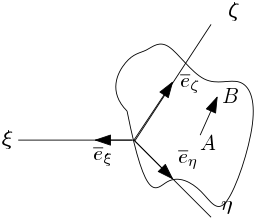
\includegraphics[width=5cm]{fig3.png} 
  \end{figure}  
  $$ \v{v_B} = \v{v_A} + [\v{\omega}, \v{AB}] $$
  
  \begin{proof}
  $$ \v{AB} = \xi \v{e_{\xi}} + \eta \v{e_{\eta}} + \zeta \v{e_{\zeta}} $$
  $$ \dot{\v{AB}} = \xi \dot{\v{e_{\xi}}} + \eta \dot{\v{e_{\eta}}} + \zeta \dot{\v{e_{\zeta}}},~~ \dot{\xi} = \dot{\eta} = \dot{\zeta} = 0 $$
  $$ \dot{\left(\v{r_B} - \v{r_A}\right)}~~ = \xi[\v{\omega}, \v{e_{\xi}}] + \eta[\v{\omega}, \v{e_{\eta}}] + \zeta[\v{\omega}, \v{e_{\zeta}}] $$ 
  $$ \dot{\v{r_B}} - \dot{\v{r_A}} = [\v{\omega}, \xi \v{e_{\xi}} + \eta \v{e_{\eta}} + \zeta \v{e_{\zeta}}] $$
  $$ \v{v_B} = \v{v_A} + [\v{\omega}, \v{AB}] $$  
  \end{proof}
  
  \begin{cor}
  $S\xi\eta\zeta \rightarrow \v{\omega}$, $S'\xi'\eta'\zeta' \rightarrow \v{\omega}'$
  $$ 
  \left.
  \begin{array}{ccc}
  \v{v_B} = \v{v_A} + [\v{\omega}, \v{AB}] \\
  \v{v_B} = \v{v_A} + [\v{\omega'}, \v{AB}]
  \end{array}
  \right|
  [\v{\omega} - \v{\omega}', \v{AB}] = 0;~ \forall A, B \text{ в абсолютно твердом теле} \Rightarrow
  $$
  $$ \Rightarrow \v{\omega} - \v{\omega}' = 0 \Rightarrow \boxed{\v{\omega} = \v{\omega}'} $$
  \end{cor}
  
  \begin{ass}(Формула Ривальса) $ \v{w_B} = \v{w_A} + [\v{\varepsilon}, \v{AB}] + [\v{\omega}, [\omega, \v{AB}]] $.
  \end{ass}
  \begin{proof}
  $$ \v{v_B} = \v{v_A} + [\v{\omega}, \v{AB}] $$
  $$ \dot{\v{v_B}} = \dot{\v{v_A}} + [\dot{\v{\omega}}, \v{AB}] + [\v{\omega}, \dot{\v{r_B} - \v{r_A}}~]  $$
  $$ \v{w_B} = \v{w_A} + [\v{\varepsilon}, \v{AB}] + [\v{\omega}, [\v{\omega}, \v{AB}]]  $$
  $$ [\v{\varepsilon}, \v{AB}] \text{ - вращательное ускорение,~~} [\v{\omega}, [\v{\omega}, \v{AB}]] \text{ - осестремительное ускорение} $$ 
  \end{proof}
  
  \subsubsection*{Геометрический смысл $\v w_{OC}$}
  \begin{figure}[H]
  \centering
  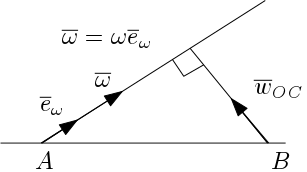
\includegraphics[width=5cm]{fig4.png} 
  \end{figure}
  $ \v{w} = [\v{\omega}, [\v{\omega}, \v{AB}]] = \v{\omega} (\v{\omega}, \v{AB}) - \v{AB} \omega^2 = \omega^2 ( \v{e_{\omega}}(\v{AB}, \v{e_{\omega}}) - \v{AB}) $
  
  $ | \v{w_{\textbf{ос}}} |= \omega^2 \rho(B, l) $
  
  \begin{ass}
  Проекции скоростей двух точек твердого тела на прямую, их соединяющую, равны.
  \begin{figure}[H]
  \centering
  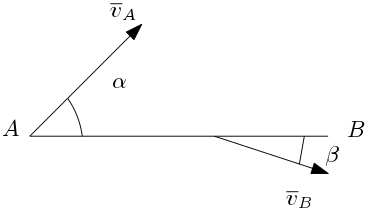
\includegraphics[width=5cm]{fig5.png} 
  \end{figure}
  \end{ass}
  \begin{proof}
  $$ \v{v_B} = \v{v_A} + [\v{\omega}, \v{AB}] $$
  $$ (\v{v_B}, \v{AB}) = (\v{v_A}, \v{AB}) + ([\v{\omega}, \v{AB}], \v{AB}) $$
  $$ v_B \cos \beta = v_A \cos \alpha $$
  \end{proof}
  \begin{ntc}
  Аналогичная теорема для ускорений не верна.
  \end{ntc}
  
  \section{Классификация движения твердого тела}
  
  \subsection{Поступательное движение}
  \begin{df}
  Такое движение твердого тела, при котором угловая скорость равна нулю.
  \end{df}
  \begin{figure}[H]
  \centering
  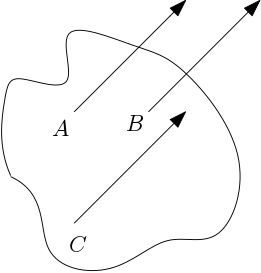
\includegraphics[width=5cm]{img/fig6.png} 
  \end{figure}
  $$ \v{v_B} \equiv \v{v_A} $$
  $$ \v{w_B} \equiv \v{w_A} $$
  \paragraph{Мгновенное поступательное движение:}
  $ \exists t : \v{\omega}(t) = 0,~~ \v{\varepsilon}(t) \neq 0 $
  
  \subsection{Вращательное движение (вращение вокруг неподвижной оси)}
  ~
  $$ \exists A, B : \v{v_A} = \v{v_B} = 0 $$
  \begin{figure}[H]
  \centering
  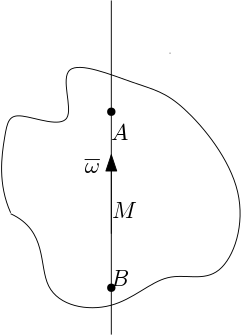
\includegraphics[width=5cm]{img/fig7.png} 
  \end{figure}
  \begin{flalign*}
  & \v{v_B} = \v{v_A} + [\v{\omega}, \v{AB}], \v{v_A} = \v{v_B} = 0 \Rightarrow [\omega, \v{AB}] = 0 \Rightarrow \omega \parallel \v{AB} &\\
  & \forall M \in l : \v{v_M} = 0 \text{, $l$ - ось вращения} &\\
  & \dot{\vec{e}}_{\xi} = \dot{\varphi} \vec{e}_{\eta},~ \dot{\vec{e}}_{\eta} = -\dot{\varphi} \vec{e}_{\xi},~ \dot{\vec{e}}_{\zeta} = 0  &\\
  & \vec{\omega} = \vec{e}_{\xi}(-\dot{\varphi}\vec{e}_{\xi}, \vec{e}_{\zeta}) + \vec{e}_{\eta}(0, \vec{e}_{\xi}) + \vec{e}_{\zeta}(\dot{\varphi} \vec{e}_{\eta}, \vec{e}_{\eta}) = \dot{\varphi} \vec{e}_{\zeta} = \dot{\varphi}\vec{e}_{z} &\\
  & \vec{\varepsilon} = \dot{\vec{\omega}} = \ddot{\varphi}\vec{e}_z &\\
  & \vec{v}_p = \vec{v}_{p'} + [\vec{\omega}, \overline{pp'}] = 0 + [\dot{\varphi}\vec{e}_z, \xi\vec{e}_{\xi} + \eta\vec{e}_{\eta}] = \dot{\varphi}(\xi\vec{e}_{\eta} - \eta\vec{e}_{\xi}) &\\
  & | \vec{v}_p | = | \vec{\omega} | \cdot | \overline{p'p} | &\\
  & \vec{w}_p = \vec{w}_{p'} + [\vec{\varepsilon}, \overline{p'p}] + [\vec{\omega}, [\vec{\omega}, \overline{p'p}]] = 0 + [\vec{\varepsilon}, \overline{p'p}] - \omega^2 \overline{p'p} &\\
  \end{flalign*}
 
  \lline{20.09.2017}  %2017-09-20
  \subsection{Плоскопараллельное движение}
  \begin{df}
  Движение твердого тела называется плоскопараллельным, если скорости всех точек тела параллельны некоторой неподвижной плоскости:
  $$ \v{v}_{p_i} \parallel \pi,~ \forall p_i \in \text{АТТ} $$
  \end{df}

  $$ \v{v}_{p_i} = \v{v}_{p_j} + [\v{\omega}, \v{p_j p_i}] $$
  $$ 
  (\v \omega, \v{v_{p_i}} - \v{v}_{p_j}) = 0 \Leftrightarrow 
  \left[
  \begin{array}{l}
  \v{\omega} = 0 \\
  \v{v}_{p_i} = \v{v}_{p_j},~ \forall p_i, p_j \in \text{АТТ} \\
  \v{\omega} \perp \v{v}_{p_i} - \v{v}_{p_i} \parallel \pi \\
  \end{array}
  \right.
  $$
  $$ \v{v}_{M_i} = \v{v}_{M_j} + [\v{\omega}, \overline{M_jM_i}] = \v{v}_{M_j} \quad \forall M_i, M_j: \overline{M_iM_j} \perp \pi \Rightarrow \v{w}_{M_i} = \v{w}_{M_j} $$
  Качение:
  $$ \v{r}_S = x_S \v{e}_x + y_S \v{e}_y $$
  $$ \dot{\v{e}}_{\xi} = \dot{\varphi}\v{e}_{\eta},~~ \dot{\v{e}}_{\eta} = \dot{\varphi}\v{e}_{\zeta},~~ \dot{\v{e}}_{\zeta} = 0$$
  $$ \v{\omega} = \dot{\varphi} \v{e}_z,~~ \v{\varepsilon} = \ddot{\varphi} \v{e}_z \parallel \v{\omega}$$
  $$ \v{v}_M = \v{v}_S + [\v{\omega}, \overline{SM}] $$
  $$ \v{w}_M = \v{w}_S + [\v{\varepsilon}, \overline{SM}] + [\v{\omega}, [\v{\omega}, \overline{SM}]] = \v{w}_s + [\v{\varepsilon}, \overline{SM}] - \omega^2 \overline{SM} $$ 

  \begin{teo}
  Если при плоскопараллельном движении угловая скорость твердого тела отлична от нуля, то существует точка, скорость которой равна нулю в данный момент времени.
  \end{teo}
  \begin{proof}
  $$
  \begin{cases}
  \v{v}_c = \v{v}_s + [\v{\omega}, \v{SC}] \\
  \v{v}_c = 0 \\
  \end{cases}
  \Rightarrow
  [\v{\omega}, \v{v}_s] + [\v{\omega}, [\v{\omega}, \v{SC}]] = 0 $$
  $$ [\v{\omega}, \v{v}_s] + \v{\omega}(\v{\omega}, \v{SC}) - \omega^2 \v{SC} = 0 $$
  $$ \v{SC} = \frac{[\v{\omega}, \v{v}_s]}{\omega^2} $$
  \end{proof}
  \begin{cor} 
  Любое плоскопараллельное движение является либо мгновенно-поступательным, либо мгновенно-вращательным
  \end{cor}
  \begin{proof}
  $\v{\omega} = 0$ - мгновенно-поступательное. $\v{\omega}(t) \neq 0$ - вращение вокруг $l$. 
  
  \end{proof}

  \begin{figure}[H]
  \centering
  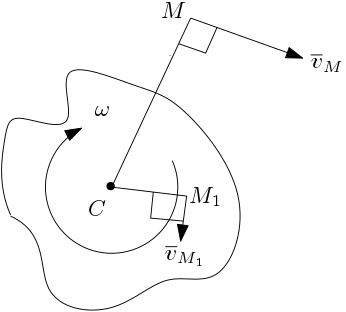
\includegraphics[width=5cm]{fig8.png} 
  \end{figure}  

  \begin{df}
  $C$ - мгновенный центр скоростей
  \end{df}
  \begin{ntc}
  Положение $C$ меняется со временем.
  \end{ntc}
  \begin{xmp}
  Качение без проскальзывания
  \end{xmp}

  \subsection{Тело с неподвижной точкой (вращение вокруг точки)}
  $$ \exists O: \v{v}_O \equiv 0 $$
  $$ l \parallel \v{\omega}, O \in l $$
  $$ \v{v}_M = \v{v}_O + [\v{\omega}, \v{OM}] = 0 + 0,~ \forall M \in l $$
  \begin{figure}[H]
  \centering
  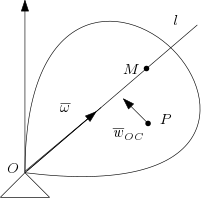
\includegraphics[width=5cm]{fig9.png} 
  \end{figure}  

  \begin{df} 
  $l$ - мгновенная ось вращения 
  \end{df}
  $$ \v{v}_p = [\v{\omega}, \v{OP}],~ \v{w_p} = [\v{\varepsilon}, \v{OP}] + \underbrace{[\v{\omega}, [ \v{\omega}, \overline{OP}]]}_{\v{v}_{OC}} $$
  \subsection{Винтовое движение}
  \begin{df} 
  Движение твердого тела называется винтовым, если тело равномерно вращается вокруг неподвижной оси, а скорости всех точек, лежащий на этой оси, равны между собой, постоянны и сонаправлены с осью.
  \end{df}
  \subsection{Общий случай}
  \begin{teo}
  $ \v{\omega} \neq 0 \Rightarrow \exists l:~ \v{\omega} \parallel l,~ \v{v}_{k_i} \parallel l,~ \forall k_i \in l$
  \end{teo}
  \begin{figure}[H]
  \centering
  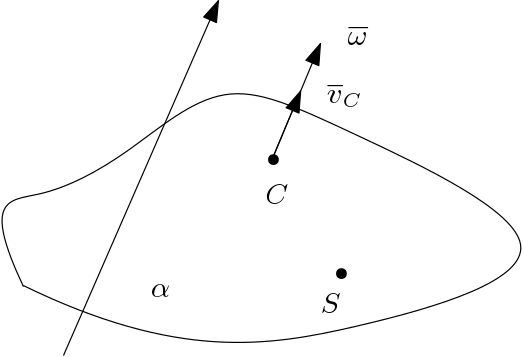
\includegraphics[width=5cm]{fig10.png} 
  \end{figure}  

  \begin{proof}
  $$ \v{\alpha} \perp \v{\omega},~ S \in \alpha $$
  $$
  \begin{cases}
  \v{v}_c = \v{v}_s + [\v{\omega}, \v{SC}] \\
  \v{v}_c = \lambda \v{\omega}
  \end{cases}
  \Rightarrow
  0 = [\v{\omega}, \v{v}_s] + [\v{\omega}, [\v{\omega}, \v{SC}]]
  $$
  $$ [ \v{\omega}, \v{v}_s] + \v{\omega}(\v{\omega}, \v{SC}) - \omega^2 \v{SC} = 0 $$
  $$ \v{SC} = \frac{[\v{\omega},\v{v}_c]}{\omega^2} $$
  $$ \exists l: C \in l, l \parallel \v{\omega} $$
  $$ \v{v}_{C_1} = \v{v}_C + [\v{\omega}, \v{CC_1}] = \v{v}_C,~~ \forall C_1 \in l$$ 

  \end{proof}
  $$\v{v}_C = \v{v}_S + \left[ \v{\omega}, \frac{[\v{\omega}, \v{v}_C]}{\omega^2} \right] = \v{v}_S + \frac{1}{\omega^2}\left(\v{\omega}(\v{\omega}, \v{v}_S) - \omega^2\v{v}_S \right) = \underbrace{\frac{(\v{\omega}, \v{v}_S)}{\omega^2}}_{\lambda} \v{\omega}$$
  $$\lambda = \frac{(\v{\omega}, \v{v}_S)}{\omega^2} \text{ - параметр (шаг винта).}$$

  \begin{cor}
  Любое движение твердого тела является в каждый момент времени либо мгновенно-поступательным ($\omega = 0$, $\lambda \rightarrow +\infty$), либо мгновенно-вращательным ($\omega \neq 0$, $\lambda = 0$) , либо мгновенно-винтовым ($\omega \neq 0$, $\lambda \neq 0$).
  \end{cor}
  \begin{df}
  $\{l, \v{\omega}, \v{v}\}$ - кинематический винт.
  \end{df}
  $$\v{v}_S = v_x\v{e}_x + v_y\v{e}_y + v_z\v{e}_z$$
  $$\v{r}_S = x_S\v{e}_x + y_S\v{e}_y + z_S\v{e}_z$$
  $$\v{\omega} = \omega_x\v{e}_x + \omega_y\v{e}_y + \omega_z\v{e}_z$$
  $$ \v{r}_C = x\v{e}_x + y\v{e}_y + z\v{e}_z $$
  $$ \v{v}_S + [\v{\omega}, \v{SC}] = \lambda \v{\omega} \Rightarrow \lambda = \frac{v_x + \omega_y(z - z_S) - \omega_z(y - y_S)}{\omega_x} = $$
  $$ = \frac{v_y + \omega_z(x - x_S) - \omega_x(z - z_S)}{\omega_y} = \frac{v_z + \omega_x(y - y_S) - \omega_y(x - x_S)}{\omega_z} $$
  

  \section{Кинематика сложного движения}
  \begin{figure}[H]
  \centering
  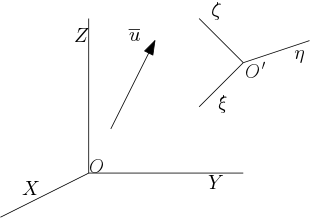
\includegraphics[width=5cm]{fig11.png} 
  \end{figure}  

  $OXYZ$ - неподвижная система отсчета ($\v{r})$, $O_1\xi\eta\zeta$ - подвижная система отсчета ($\v{\rho}$).

  $$ \v{u} = u_x \v{e}_x + u_y \v{e}_y + u_z \v{e}_z $$
  $$ \v{u} = u_{\xi} \v{e}_{\xi} + u_{\eta} \v{e}_{\eta} + u_{\zeta} \v{e}_{\zeta} $$
  $$ \frac{d\v{u}}{dt} = \dot {u_x} \v{e}_x + \dot{u_y} \v{e}_y + \dot{u_z} \v{e}_z \text{ - абсолютная производная} $$
  $$ \dot{\v u} = \dot{u_{\xi}} \v{e}_{\xi} + \dot{u_{\eta}} \v{e}_{\eta} + \dot{u_{\zeta}} \v{e}_{\zeta} \text{ - относительная производная}$$
  \begin{teo}(Связь абсолютной и относительной производной) 
  $\frac{d\v{u}}{dt} = \dot{\v{u}} + [\v{\omega}, \v{u}]$, где $\v{\omega}$ - угловая скорость $O_1\xi\eta\zeta$ относительно $OXYZ$
  \end{teo}
  \begin{proof}
  $$ \frac{du}{dt} = \dot{u}_{\xi}\v{e}_{\xi} + \dot{u}_{\eta}\v{e}_{\eta} + \dot{u}_{\zeta}\v{e}_{\zeta} + u_{\xi}\frac{d\v{e}_{\xi}}{dt} + u_{\eta}\frac{d\v{e}_{\eta}}{dt} + u_{\zeta}\frac{d\v{e}_{\zeta}}{dt} = $$
  $$ = \dot{\v{u}} + u_{\xi}[\v{\omega}, \v{e}_{\xi}] + u_{\eta}[\v{\omega}, \v{e}_{\eta}] + u_{\zeta}[\v{\omega}, \v{e}_{\zeta}] = \dot{\v{u}} + [\v{\omega}, \v{u}] $$
  $$ \left(\frac{d\v{e}_i}{dt} = [\v{\omega}, \v{e}_i] - \text{ - формула Пуассона},~~ \dot{\v{e}}_i = 0\right) $$
  \end{proof}
  \subsection{Сложное движение материальной точки}
  \begin{figure}[H]
  \centering
  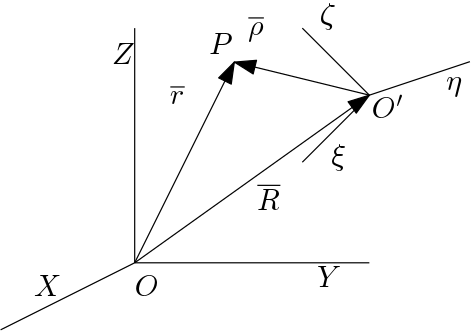
\includegraphics[width=5cm]{fig12.png} 
  \end{figure}
  \begin{df}
  Абсолютной скоростью материальной точки называется ее скорость относительно неподвижной системы отсчета. $\v{v}_{\text{абс}} = \frac{d}{dt}\v{r}$
  \end{df}
  \begin{df}
  Относительной скоростью материальной точки называется ее скорость относительно подвижной системы отсчета. $\v{v}_{\text{отн}} = \dot{\v{\rho}}$
  \end{df}
  \begin{df}
  Переносной скоростью материальной точки называется абсолютная скорость той точки подвижной системы отсчета, в которой находится движующаяся точка в данный момент времени.
  \end{df}
  \begin{teo}
  [Формула сложения скоростей] $\v{v}_{\text{абс}} = \v{v}_{\text{отн}} + \v{v}_{\text{пер}}$
  \end{teo}
  \begin{proof}
  $$ \v{v}_{\text{абс}} = \frac{d}{dt}(\v{R} + \v{\rho}) = \frac{dR}{dt} + \dot{\v{\rho}} + [\v{\omega}, \v{\rho}] = $$
  $$ = \v{v}_{O_1} + \v{v}_{\text{отн}} + [\v{\omega}, \v{\rho}] = \v{v}_{\text{отн}} + \v{v}_{\text{пер}} $$
  \end{proof}
  \begin{df}
  Абсолютным ускорением материальной точки называется ее ускорение относительно неподвижной системы отсчета. $\v{w}_{\text{абс}} = \frac{d}{dt}\v{v}_{\text{абс}}$
  \end{df}
  \begin{df}
  Относительным ускорением материальной точки называется ее ускорение относительно подвижной системы отсчета. $\v{w}_{\text{отн}} = \dot{\v{v}_{\text{отн}}}$
  \end{df}
  \begin{df}
  $ \v{w}_{\text{пер}} = \v{\omega}_{O_1} + [\v{\varepsilon}, \v{\rho}] + [\v{\omega}, [\v{\omega}, \v{\rho}]] $
  \end{df}
  \begin{df}
  $ \v{w}_{\text{кор}} = 2[\v{\omega}, \v{v}_\text{отн}] $
  \end{df}
  \begin{teo}
  [Формула сложения ускорений] $\v{w}_{\text{абс}} = \v{w}_{\text{отн}} + \v{w}_{\text{пер}} + \v{w}_{\text{кор}}$
  \end{teo}

  \begin{proof}
  $$ \v{w}_{\text{абс}} = \frac{d}{dt}(\v{v}_{\text{отн}} + \v{v}_{\text{пер}}) = \frac{d}{dt} (\v{v}_{\text{отн}} + \v{v}_{O_1} + [\v{\omega}, \v{\rho}]) = $$ 
  $$ = \dot{\v{v}}_{\text{отн}} + [\v{\omega}, \v{v}_{\text{отн}}] + \frac{d}{dt}\v{v}_{O_1} + \left[\frac{d\v{\omega}}{dt}, \v{\rho}\right] + [\v{\omega}, \v{\rho} + [\v{\omega}, \v{\rho}]] = $$ 
  $$ = \dot{\v{v}}_{\text{отн}} + \dot{\v{v}}_{O_1} + [\v{\varepsilon}, \v{\rho}] + 2[\v{\omega}, \v{v}_{\text{отн}}] + [\v{\omega}, [\v{\omega}, \v{\rho}]] $$
  \end{proof}
  \lline{27.09.2017}  %2017-09-27
  \subsection{Сложное движение твердого тела}
  Рассмотрим неподвижную систему отсчета $OXYZ$, подвижную $O_1xyz$, и систему, связанную с телом $S\xi\eta\zeta$.
  \begin{df} Абсолютная угловая скорость - угловая скорость $S\xi\eta\zeta$ относительно $OXYZ$\end{df}
  \begin{df} Относительная угловая скорость - угловая скорость $S\xi\eta\zeta$ относительно $O_1xyz$\end{df}
  \begin{df} Переносная угловая скорость - угловая скорость $Oxyz$ относительно $OXYZ$\end{df}  
  \begin{teo}[О сложении угловых скоростей] $\v{\omega}_{\text{абс}} = \v{\omega}_{\text{отн}} + \v{\omega}_{\text{пер}}$ \end{teo}
  \begin{proof}
  $$ \v{v}_A^{\text{абс}} = \v{v}_A^{\text{отн}} + \v{v}_A^{\text{пер}} $$
  $$ \v{v}_B^{\text{абс}} = \v{v}_B^{\text{отн}} + \v{v}_B^{\text{пер}} $$
  $$ \v{v}_B^{\text{абс}} = \v{v}_A^\text{абс} + [\v{\omega}_{\text{абс}}, \overline{AB}] $$

  $$ \v{v}_B^{\text{отн}} = \v{v}_A^\text{отн} + [\v{\omega}_{\text{отн}}, \overline{AB}] $$

  $$ \v{v}_B^{\text{пер}} = \v{v}_A^\text{пер} + [\v{\omega}_{\text{пер}}, \overline{AB}] $$
  $$ \Rightarrow 0 = 0 + [\v{\omega}_{\text{абс}} - \v{\omega}_{\text{отн}} - \v{\omega}_{\text{пер}}, \overline{AB}] = 0,~~ \forall \overline{AB} \Leftrightarrow \v{\omega}_{\text{абс}} = \v{\omega}_{\text{отн}} + \v{\omega}_{\text{пер}} $$
  \end{proof}

  \begin{ntc}
  $\frac{d\v{\omega}_{\text{пер}}}{dt} = \dot{\v{\omega}}_\text{пер} + [\v{\omega}_\text{пер}, \v{\omega}_\text{пер}] = \dot{\v{\omega}}_\text{пер} $
  \end{ntc}

  \begin{teo}[О сложении угловых ускорений] 
  $\v{\varepsilon}_{\text{абс}} = \v{\varepsilon}_{\text{отн}} + \v{\varepsilon}_{\text{пер}} + [\v{\omega}_{\text{пер}}, \v{\omega}_\text{отн}]$, где $\v{\varepsilon}_{\text{абс}} = \frac{d}{dt}\v{\omega}_{\text{абс}}$, $\v{\varepsilon}_{\text{отн}} = \dot{\v{\omega}}_{\text{отн}}$, $\v{\varepsilon}_{\text{пер}} = \frac{d}{dt}\v{\omega}_{\text{пер}} = \dot{\v{\omega}}_{\text{пер}}$
  \end{teo}

  \begin{proof}
  $$ \v{\varepsilon}_{\text{абс}} = \frac{d}{dt}(\v{\omega}_{\text{отн}} + \v{\omega}_{\text{пер}}) = $$ 
  $$ = \dot{\v{\omega}}_{\text{отн}} + [\v{\omega}_{\text{пер}}, \v{\omega}_{\text{отн}}] + \frac{d}{dt}\v{\omega}_{\text{пер}} =
  \v{\varepsilon}_{\text{отн}} + [\v{\omega}_{\text{пер}}, \v{\omega}_{\text{отн}}] + \v{\varepsilon}_{\text{пер}} $$ 

  \end{proof}

  \subsubsection{Несколько подвижных систем отсчета}~
  
  \noindent $OXYZ$ - неподвижная СО \\
  $Ox_1y_1z_1$, $Ox_2y_2z_2$ , $\ldots Ox_ny_nz_n$ - подвижные СО \\
  $S\xi\eta\zeta$ - связана с телом \\
  $\v{\omega}$ - угловая скорость $S\xi\eta\zeta$ относительно $OXYZ$ \\
  Тогда: $\v{\omega} = \sum\limits_{i = 1}^{n} \v{\omega_i}$
  
  \subsection{Кинематические формулы Эйлера}
  \begin{figure}[H]
  \centering
  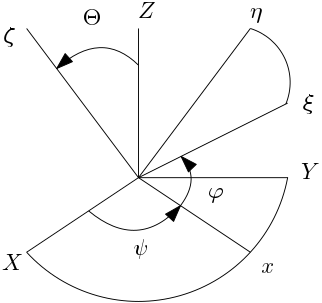
\includegraphics[width=5cm]{fig13.png} 
  \end{figure}  

  \begin{df} $ Ox = (OXY)\cap(O\xi\eta) $ - линия узлов \end{df}
  \begin{df} $\psi = \angle(Ox, OX)$ - угол прецессии \end{df}
  \begin{df} $\Theta = \angle (O\zeta, OZ)$ - угол нутации \end{df}
  \begin{df} $\varphi = \angle (Ox, O\xi)$ - угол собственного вращения \end{df}
  \begin{df} $\{\psi, \Theta, \varphi\}$ - углы Эйлера \end{df}

  Повороты:
  $ OXYZ \xrightarrow{\psi, OZ} OxyZ \xrightarrow{\Theta, Ox} Oxy\zeta \xrightarrow{\varphi, O\zeta} O\xi\eta\zeta $

  $\v{\omega} = \dot{\psi}\v{e}_Z + \dot{\Theta}\v{e}_x + \dot{\varphi}\v{e}_{\zeta}$

  $\v{e}_x = \cos \varphi \v{e}_{\xi} - \sin \varphi \v{e}_{\eta}$
  
  $\v{e}_z = \cos \Theta \v{e}_{\zeta} + \sin \Theta ( \sin \varphi \v{e}_{\xi} + \cos \varphi \v{e}_{\eta} )$
  $$\begin{array}{rcl}\v{\omega} & = & \dot\psi(\sin \Theta \sin \varphi \v{e}_{\xi} + \sin \Theta \cos \varphi \v{e}_{\eta} + \cos \Theta \v{e}_{\zeta}) \\
  & + & \dot \Theta (\cos \varphi \v{e}_{\xi} - \sin \varphi\v{e}_{\eta}) \\
  & + & \dot{\varphi}\v{e}_{\zeta} = \omega_{\xi}\v{e}_{\xi} + \omega_{\eta}\v{e}_{\eta} + \omega_{\zeta}\v{e}_{\zeta} \\
  \end{array}$$

  $$
  \begin{cases}
  \v{\omega}_{\xi} = \dot{\psi}\sin\Theta \sin\varphi + \dot{\Theta}\cos\varphi \\
  \v{\omega}_{\eta} = \dot{\psi}\sin\Theta \cos\varphi - \dot{\Theta}\sin\varphi \\
  \v{\omega}_{\zeta} = \dot{\psi}\cos\Theta + \dot{\varphi} \\
  \end{cases}
  \text{ - кинематические формулы Эйлера}
  $$

  \begin{df} 
  Движение твердого тела называется прецессией, если некоторая ось, неподвижная в теле, в абсолютном пространстве движется по поверхности неподвижного кругового конуса. $\dot{\Theta} = 0$. Если $\dot {\psi} = const$, $\dot {\varphi} = const$, то прецессия называется регулярной.
  \end{df}

  \section{Алгебра кватернионов}
  \begin{df} Алгеброй над полем называется векторное пространство над этим полем, снабженное билинейной операцией умножения. \end{df}
  \begin{xmp} ~

  $\underline{n=2}$(\textit{Комплексные числа}). $z_1 = a + bi$, $z_2 = c + di$ 

  $$ z_1z_2 = (ac - bd) + (ad + bc)i $$

  \end{xmp}
  $\underline{n=4}$(\textit{Алгебра кватернионов})

  \begin{flalign*}
  & \Lambda = \lambda_0 \v{i}_0 + \lambda_1 \v{i}_1 + \lambda_2 \v{i}_2 + \lambda_3 \v{i}_3 \in \mathbb{H} &\\
  & \{\v{i}_0, \v{i}_1, \v{i}_2, \v{i}_3\} \text{ - базис} &\\ 
  & \Lambda = \lambda_0 + \overline{\lambda} &\\
  & i_0 \circ i_k = i_k \quad k = \overline{1, 3},~ i_0 \circ i_0 = 1 &\\
  & i_k \circ i_m = -(i_k, i_m) + [i_k, i_m] \quad k, m \in \{1,2,3\}, \qquad  \text{В частности, $i_k \circ i_k = -1$}&\\
  & \overline{\lambda} \circ \overline{\mu} = (\lambda_1 \v{i}_1 + \lambda_2 \v{i}_2 + \lambda_3 \v{i}_3) \circ (\mu_1 \v{i}_1 + \mu_2 \v{i}_2 + \mu_3 \v{i}_3) = -(\overline{\lambda}, \overline{\mu}) + [\overline{\lambda}, \overline{\mu}] &\\
  & \Lambda \circ M = (\lambda + \overline{\lambda}) \circ (\mu + \overline{\mu}) = \lambda_0 \mu_0 + \lambda_0\overline{\mu} + \overline{\lambda}\mu_0 - (\overline{\lambda}, \overline{\mu}) + [\overline{\lambda}, \overline{\mu}] &\\
  \end{flalign*}
  \paragraph{Свойства:}
  \begin{enumerate}
    \item $(\Lambda \circ M) \circ N = \Lambda \circ (M \circ N)$
    \item $(\Lambda + M) \circ N = \Lambda \circ N + M \circ N $
    \item $\Lambda \circ M \neq M \circ \Lambda$
  \end{enumerate}


  \lline{04.10.2017}  \begin{df}
  \[ \overline{\Lambda} = \lambda_0 - \overline{\lambda} \]
  \end{df}
  \begin{ass}
  \[ \overline{\Lambda \circ M} = \overline{M} \circ \overline{\Lambda} \]
  \end{ass}
  \begin{proof}
  \[ \overline{\Lambda \circ M} = \lambda_0\mu_0 - (\overline\lambda, \overline\mu) - \lambda_0\overline\mu - \mu_0\overline\lambda - [\overline\lambda, \overline\mu] = \]
  \[ = (\mu_0 - \overline\mu) \circ (\lambda_0 - \overline\lambda) = \overline M \circ \overline \Lambda \]
  \end{proof}
  \begin{df}
  \[ \parallel \Lambda \parallel = \Lambda \circ \overline \Lambda = (\lambda_0 + \overline \lambda) \circ (\lambda_0 - \overline \lambda) = \lambda_0^2 + \overline \lambda^2 = \sum\limits_{k = 0}^3 \lambda_k^2 = | \Lambda |^2 \text{ - норма $\Lambda$ }\]
  \end{df}
  \begin{ass}
  \[ \parallel \Lambda \circ M \parallel = \norm{\Lambda} \cdot \norm{M} \]
  \end{ass}
  \begin{proof}
  \[ \norm{\Lambda \circ M} = (\Lambda \circ M) \circ (\overline{\Lambda \circ M}) = \Lambda \circ \underbrace{M \circ \overline M}_{\norm{M}}  \circ \overline \Lambda = \norm{M} \cdot \norm{\Lambda} \]
  \end{proof}
  \begin{df}
  \[ \Lambda^{-1} = \frac{\overline \Lambda}{\norm{\Lambda}},~ \norm \Lambda \neq 0 \]
  \end{df}
  \begin{ntc}
  \[ \Lambda \circ \frac{\overline{\Lambda}}{\norm{\Lambda}} = \frac{\overline \Lambda}{\norm \Lambda} \circ \Lambda = \frac{\norm \Lambda}{\norm \Lambda} = 1 \]
  \end{ntc}

  \paragraph*{Формула Муавра}
  \begin{flalign*}
  & \Lambda = \lambda_0 + \overline \lambda =  \abs \Lambda \lb \frac{\lambda_0}{\abs \Lambda} + \frac{\overline \lambda}{\abs \lambda } \frac{\abs {\overline \lambda}}{\abs \Lambda} \rb = \abs \Lambda \lb \cos \nu + \overline e \sin \nu \rb &\\
  & \overline e = \frac{\overline \lambda}{\abs {\overline \lambda}},~ \cos\nu = \frac{\lambda_0}{\abs{\Lambda}},~ \sin\nu = \frac{\abs{\overline \lambda}}{\abs{\Lambda}} &\\
  & \Lambda_1 = \abs{\Lambda_1}(\cos \nu_1 + \overline e \sin \nu_1) &\\
  & \Lambda_2 = \abs{\Lambda_2}(\cos \nu_2 + \overline e \sin \nu_2) &\\
  & \Lambda_1 \circ \Lambda_2 = \abs{\Lambda_1}\cdot\abs{\Lambda_2}(\cos\nu_1 \cos\nu_2 - \sin\nu_1\sin\nu_2(\overline e, \overline e) + \cos\nu_1\sin\nu_2 \overline e + &\\ 
  & + \cos\nu_2\sin\nu_1\overline e + \sin\nu_2\sin\nu_2[\overline e, \overline e]) = \abs{\Lambda_1}\abs{\Lambda_2} \cdot (\cos(\nu_1 + \nu_2) + \overline e \sin(\nu_1 + \nu_2)) &\\
  \end{flalign*}
  \[ \Lambda^k = \abs \Lambda^k \cdot (\cos k\nu + \overline e \sin k\nu) \text{ --- формула Муавра } \]
  \section{Задание ориентации твердого тела с помощью кватернионов}
  $E = \{\ea, \eb, \ec\}$ --- неподвижный базис \\
  $E' = \{\ea', \eb', \ec' \}$ --- связанный с телом
  \begin{teo}
  Произвольному положению твердого тела с неподвижной точкой соответствует нормированный кватернион, удовлетворяющий равенству:
  \[ \v{e}_i' = \Lambda \circ \v{e}_i \circ \overline \Lambda,~~ i = 1\ldots3  \]
  \end{teo}
  \begin{ntc}
  $\Lambda$ --- нормирован, если $\norm \Lambda = 1$
  \end{ntc}
  \begin{proof}~
  \begin{enumerate}
  \item Нормированность
  \[ \norm{\ei'} = \norm \Lambda \cdot \norm{\ei} \cdot \norm{\overline{\Lambda}} \Rightarrow 1 = \norm \Lambda \cdot 1 \cdot \norm \Lambda \Rightarrow \norm \Lambda = 1 \]
  \item Существование решения. $\Lambda = \lambda_0 + \overline \lambda$
  \begin{flalign*}
  & 
  \begin{cases} 
  \lambda_0^2 + \overline \lambda^2 = 1  \\
  \ei' \circ \Lambda = \Lambda \circ \ei \\
  \end{cases}
  &
  \begin{cases}
  \lambda_0^2 + \overline \lambda^2 = 1 \\
  \ei' \circ (\lambda_0 + \overline \lambda) = (\lambda_0 + \overline \lambda) \circ \ei \\
  \end{cases}
  \end{flalign*}
  \begin{flalign*}
  &
  \begin{cases}
  \lambda_0 \ei' - (\ei', \overline \lambda) + [\ei', \overline \lambda] = \lambda_0\ei' - (\lambda, \ei') + [\overline \lambda, \ei] \\
  \lambda_0^2 + \overline \lambda^2 = 1 \\
  \end{cases}
  &\\
  \end{flalign*}
  \begin{flalign*}
  & \begin{cases}
  \lambda_0^2 + \overline \lambda^2= 1  \\
  (\overline \lambda, \overline r_i) = 0 \\
  \lambda_0 \overline r_i - [\overline \lambda, \overline s_i] = 0 \\
  \end{cases}
  &
  \overline r_i = \ei' - \ei,~ \overline s_i = \ei' + \ei & ~~i = 1 \ldots 3
  &\\
  \end{flalign*}
  \begin{enumerate}
  \item 
  \begin{flalign*}
  & (\overline r_k, \overline s_k) = (\ek' - \ek, \ek' + \ek) = (\ek', \ek') - (\ek, \ek) = 0 &\\
  & (\overline r_k, \overline s_l) = (\ek' - \ek, \el' + \el) = (\ek', \el') + (\ek', \el) -  (\ek, \el') - (\ek, \el) = &\\
  & = -(\el' - \el, \ek' + \ek) = -(\overline s_k, \overline r_l),~ k \neq l &\\
  \end{flalign*}
  \item \label{two.o}
  \begin{flalign*}
  & (\overline r_1, \overline r_2, \overline r_3) = (\ea' - \ea, \eb' - \eb, \ec' - \ec) = (\ea', \eb', \ec') - (\ea, \eb, \ec) - &\\ 
  & - (\ea', \eb', \ec) + (\ea, \eb, \ec') =  1 - 1 - (\underbrace{[\ea', \eb']}_{\ec'}, \ec) + (\underbrace{[\ea, \eb]}_{\ec}, \ec') = 0 &\\
  \end{flalign*}
  \item 
  \begin{flalign*}
  & \overline r_1(\overline s_2, \overline r_3) + \overline r_2(\overline s_3, \overline r_1) + \overline r_3(\overline s_1, \overline r_2) &\\
  & \re{two.o} \Rightarrow c_1\v r_1 + c_2\v r_2 + c_3\v r_3 = 0 &\\
  & 
  \begin{cases}
  0 + c_2(\v s_1, \v r_2) - c_3(\v s_2, \v r_1) = 0 \\
  -c_1(\v s_1, \v r_2) + 0 + c_3(\v s_2, \v r_3) = 0 \\
  c_1(\v s_3, \v r_1) - c_2 (\v s_2, \v r_3) + 0 = 0 \\    
  \end{cases}
  &\\
  &
  \begin{cases}
  c_1 = (\v s_2, \v r_3) \\
  c_2 = (\v s_3, \v r_1) \\
  c_3 = (\v s_1, \v r_2) \\
  \end{cases}
  \begin{cases}
  \lambda_0^2 + \lambda^2 = 1 \\
  (\v r_k, \v \lambda) = 0 \\
  \lambda_0\v r_k + [\v s_k, \v \lambda] = 0 \\
  \end{cases}
  \begin{array}{c}
  (1) \\ (2) \\ (3) \\
  \end{array}
  &\\
  &
  (3) \Leftrightarrow
  \begin{cases}
  \lambda_0\v r_1 + [\v s_1, \alpha[\v r_1, \v r_2]] = 0 \\
  \lambda_0\v r_2 + [\v s_2, \alpha[\v r_1, \v r_2]] = 0 \\
  \lambda_0\v r_3 + [\v s_3, \alpha[\v r_1, \v r_2]] = 0 \\
  \end{cases}
  &\\
  &
  \begin{cases}
  \lambda_0 \v r_1 + \alpha \v r_1 (\v s_1, \v r_1) - 0 = 0 \\
  \lambda_0 \v r_2 + 0 - \alpha\v r_2(\v s_2, \v r_1) = 0 \\
  \lambda_0 \v r_3 + \alpha r_1(\v s_3, \v r_2) - \alpha r_2(\v s_3, \v r_1) = 0 \\
  \end{cases}
  &\\
  &
  \begin{cases}
  \lambda_0\v r_1 + \alpha\v r_1(\v s_1,\v r_2) = 0 \\
  \lambda_0\v r_2 + \alpha\v r_2(\v s_1,\v r_2) = 0 \\
  \lambda_0\v r_3 + \alpha\v r_3(\v s_1,\v r_2) = 0 \\
  \end{cases}
  &
  \lambda_0 = -\alpha(\v s_1, \v r_2) = \alpha(\v s_2, \v r_1)
  &\\
  &
  (1) \Rightarrow \alpha^2((\v s_2, \v r_1)^2 + [\v r_1, \v e_2]^2)^2 = 1 \Rightarrow & \alpha = \pm \frac{1}{\sqrt{(\v s_2, \v r_1)^2 + [\v r_1, \v r_2]^2}} 
  &\\
  \end{flalign*}
  \[ \Lambda = \pm \frac{(\v s_2, \v r_1) + [\v r_1, \v r_2]}{\sqrt{(\v s_2, \v r_1)^2 + [\v r_1, \v r_2]^2}} \]
  \end{enumerate}
  \end{enumerate}
  \end{proof}
  \begin{df}
  \[ f(M) = \Lambda \circ M \circ \overline \Lambda;~~ M \rightarrow f(M),~~ \norm{\Lambda} = 1 \text{--- присоединенное преобразование} \]
  \end{df}
  \begin{ass}
  Присоединенное преобразование не меняет скалярные части кватернионов и модуль векторной части
  \end{ass}
  \begin{proof}~
  \begin{enumerate}
  \item
  $ f(M) = \Lambda \circ (\mu_0 + \overline \mu) \circ \overline \Lambda = \Lambda \circ \mu_0 \circ \overline \Lambda + \Lambda \circ \overline \mu \circ \Lambda = \mu_0 \norm \Lambda + f(\v \mu) = \mu_0 + \v \mu ' $
  \item $\mu_0^2 + \v \mu^2 = \norm M = \norm{\Lambda \circ M \circ \v \Lambda} = \norm{f(M)} = \mu_0^2 + \v \mu'^2 \Rightarrow \mu^2 = \v \mu'^2$
  \end{enumerate}
  \end{proof}
  \begin{cor}
  Всегда существует присоединенное преобразование, переводящее орты неподвижного базиса в орты базиса, связанного с телом.
  \end{cor}
  \begin{proof}
  \begin{flalign}
  & \ei' = \Lambda \circ \ei \circ \v \Lambda = f(\ei) &\\
  & \v r = \sum\limits_{k = 1}^3 r_k \ek,~~ f(r) = \Lambda \circ \sum r_k \ek \v \Lambda = \sum\limits_k r_k f(\ek) = \sum\limits_k = r_k\ek = \v r ' &\\
  \end{flalign}
  \end{proof}
  \begin{equation}
  \label{b.star}
  \boxed{\v r' = \Lambda \circ \v r \circ \v \Lambda}
  \end{equation}
  \begin{cor}
  При повороте твердого тела вокруг неподвижной точки справедлива \re{b.star}, где $\v r$ -- начальное положение точки, $\v r'$ -- ее положение после поворота, а $\Lambda$ -- кватернион соответствующего преобразования.
  \end{cor}
  \lline{11.10.2017}  %2017-10-11
  \begin{teo}
  Преобразование, заданное кватернионом $\Lambda = \cos \nu + \v e \sin \nu$ соответствует повороту пространства вокруг вектора $\v e$ на угол $2\nu$
  \end{teo}
  \begin{proof}~
  \begin{enumerate}
  \item 
  \begin{flalign*}
  & \Lambda = \lambda_0 + \v \lambda &\\
  & \v \lambda' = f(\v \lambda) = \Lambda \circ \v \lambda \circ \v \Lambda = (\lambda_0 + \v \lambda) \circ \v \lambda \circ (\lambda_0 - \v \lambda) = &\\
  \end{flalign*}
  \begin{flalign*}
  & (\lambda_0 + \v \lambda) \circ (- \lambda^2 + \lambda_0 \v \lambda) = -\lambda_0\v \lambda ^2 - \lambda_0\v \lambda ^2 + \lambda_0^2 + \lambda_0^2 \v \lambda = &\\
  & = \v \lambda(\lambda_0^2 + \v \lambda^2) \Rightarrow \v \lambda \text{ --- неподвижная ось} \Rightarrow &\\
  & \Rightarrow \v e = \frac{\v \lambda}{\sin \nu} \text{ --- ось поворота} &\\
  & \v a \in \pi \perp \v e &\\
  & \v a' = f(\v a) = (\cos \nu + \v e \sin \nu) \circ \v a \circ (\cos \nu - \v e \sin \nu) = &\\
  & = (\cos \nu + \v e \sin \nu ) \circ ([\v a, \v e] \cdot \sin \nu + \cos \nu \v a - \sin \nu [\v a, \v e]) = &\\
  & \cos^2 \nu \v a + \cos \nu \sin \nu (\v a, \v e) + \cos\nu \sin\nu = \ldots &\\
  \end{flalign*}
  \item
  \begin{flalign*}
  & \overline a' = ((\cos \frac{\varphi}{2} + \v e\sin\frac{\varphi}{2}) \circ \overline a) \circ (\cos \frac{\varphi}{2} + \overline e \sin \frac{\varphi}{2}) = &\\ 
  & = (\overline a \cos \frac{\varphi}{2} + [\overline e, \overline a] \sin \frac{\varphi}{2}) \circ (\cos \frac{\varphi}{2} - \overline e \sin\frac{\varphi}{2}) = &\\ 
  & = \overline a \cos^2 \frac{\varphi}{2} + 2[\overline e, \overline a]\cos\frac{\varphi}{2}\sin\frac{\varphi}{2} - \overline a \sin^2 \frac{\varphi}{2} = &\\ 
  & = \overline a \cos \varphi + [\overline e, \overline a]\sin \varphi &\\
  \end{flalign*} 
  \[ \abs {\overline a'} = \abs{\overline a} \]
  \end{enumerate}
  \end{proof}  
  \begin{cor}
  \[ \Lambda = \lambda_0 + \lambda_1\ea + \lambda_2\eb + \lambda_3\ec = \lambda_0 + \lambda_1\ea' + \lambda_2\eb' + \lambda_3\ec' \]
  \end{cor}
  \begin{df}
  \[\lambda_0,~ \lambda_1,~ \lambda_2,~ \lambda_3 \text{ --- Параметры Родрига-Гамильтона}\]
  \end{df}
  \begin{cor}[Теорема Эйлера о конечном повороте]
  Любые два положения твердого тела с неподвижной точкой могут быть получены одно из другого одним поворотом вокруг некоторой оси, проходящей через неподвижную точку на некоторый угол
  \end{cor}
  \begin{proof}~
  \begin{enumerate}
  \item \[ \forall E, E'~~ \exists \Lambda:\; E \rightarrow E'\]
  \item \[ \forall \Lambda \overline r \rightarrow \overline r' \Leftrightarrow \text{Поворот вокруг $e$ на $\varphi$} \]
  \end{enumerate}
  \end{proof}
  \begin{flalign*}
  & E \xrightarrow{\Lambda_1} E' \xrightarrow{\Lambda_2} E'',~ E \xrightarrow{\Lambda} &\\
  & \overline r' = \Lambda_1 \circ \overline r \circ \overline \Lambda,~ \overline r'' = \Lambda_2 \circ \overline r' \circ \overline \Lambda &\\
  & \overline r'' = \Lambda_2 \circ \Lambda_1 \circ \overline r \circ \overline \Lambda \circ \overline \Lambda_2 = \Lambda \circ \overline r \circ \overline \Lambda,~~ \Lambda = \Lambda_2 \circ \Lambda_1 &\\
  \end{flalign*}

  \[ \boxed{\Lambda = \Lambda_2 \circ \Lambda_1} \text{ --- формула сложения поворотов} \]

  \begin{flalign*}
  & \Lambda_2 = \lambda_0^{(2)} + \sum\limits_{k=1}^{3} \lambda_k^{(2)} \overline e_k'' = \lambda_0^{(2)} +  \sum\limits_{k=1}^{3} \lambda_k^{(2)} \overline e_k' &\\
  & \Lambda_2^* = \lambda_0^{(2)} + \sum\limits_{k=1}^{3} \lambda_k^{(2)}\overline e_k \text{ --- собственный к $\Lambda_2$ кватернион} &\\
  & \overline e_k' = \Lambda_1 \circ \overline e_k \circ \overline \Lambda_1,~~ \Lambda_2  =\lambda_0^{(2)} + \sum\lambda_k^{(2)}\Lambda_1 \circ \overline  e_k  \circ \overline \Lambda_1 = &\\
  & = \Lambda_1 \circ (\lambda_0^{(2)} + \sum \lambda_k^{(2)} \overline e_k) \circ \overline \Lambda_1 = \Lambda_1 \circ \Lambda_2^* \circ \overline \Lambda_1 &\\
  & \Lambda = \Lambda_2 \circ \Lambda_1 = \Lambda_1 \circ \Lambda_2^* \circ (\overline \Lambda_1 \circ \Lambda_1) = \Lambda_1^* \circ \Lambda_2^*,~~ \Lambda_1^* = \Lambda_1
  \end{flalign*}

  \[ \boxed{\Lambda = \Lambda_1^* \circ \Lambda_2^*} \]
  --- формула сложения поворотов в параметрах Родрига-Гамильтона

  \section{Кинематика твердого тела в кватернионном описании}
  \begin{teo}
  Угловая скорость твердого тела определяется равенством:
  \[ \overline \omega = 2\dot \Lambda \circ \overline \Lambda \]
  где $\Lambda$ - кватернион, задающий положение твердого тела относительно неподвижного базиса
  \end{teo}
  \begin{proof}~
  \begin{enumerate}
  \item 
  \begin{flalign*}
  & B = \dot{\Lambda} \circ \overline \Lambda &\\
  & B + \overline B = \dot \Lambda \circ \overline \Lambda + \overline {\left( \dot \Lambda \circ \overline \Lambda \right)} = \dot \Lambda \circ \overline \Lambda + \Lambda \circ \dot {\overline \Lambda} = &\\ 
  & = \frac{d}{dt}(\Lambda \circ \overline \Lambda) = \frac{d}{dt}(\norm \Lambda) = 0 \Rightarrow B = -\overline B &\\
  \end{flalign*}
  \item 
  \begin{flalign*}
  & \dot{\overline e}_k' = [\overline \omega, \overline e_k] &\\
  & \overline e_k' = \Lambda \circ \overline e_k \circ \overline \Lambda,~~ \overline e_k = \overline \Lambda \circ \overline e_k' \circ \Lambda  &\\
  & \dot{\overline e}_k' = \dot \Lambda \circ \overline e_k \circ \Lambda + \Lambda \circ \overline e_k \circ \dot{\overline \Lambda} =  &\\
  & \dot \Lambda \circ (\overline \Lambda \circ \overline e_k' \circ \Lambda) \circ \overline \Lambda + \Lambda \circ (\overline \Lambda \circ \overline e_k' \circ \Lambda) \circ \dot{\overline \Lambda} = &\\
  & = \dot \Lambda \circ \overline \Lambda \circ \overline e_k' + \overline e_k' \circ \Lambda \circ \dot{\overline \Lambda} = B \circ \overline e_k' + \overline e_k' \circ \overline B = &\\
  & [2\overline B, \overline e_k] \Rightarrow 2\overline B = \overline \omega &\\
  \end{flalign*}
  \end{enumerate}
  \end{proof}
  \begin{xmp}
  \[ \Lambda = \cos \frac{\varphi}{2} + \overline e \sin \frac{\varphi}{2} \]
  \begin{flalign*}
  & \overline \omega = 2(-\sin \frac{\varphi}{2} \cdot \frac{\dot \varphi}{2} + \dot{\overline e}\sin\frac{\varphi}{2} + \overline e \cos \frac{\varphi}{2} \cdot \frac{\dot \varphi}{2}) \circ (\cos \frac{\varphi}{2} + \overline e \sin \frac{\varphi}{2}) = &\\
  & =\cos \frac{\varphi}{2} \cdot \sin \frac{\varphi}{2} \cdot \dot \varphi+ \cos \frac{\varphi}{2} \cdot \sin \frac{\varphi}{2} \cdot \dot \varphi + \overline e \sin^2 \frac{\varphi}{2} \cdot \dot \varphi \:+ &\\ 
  & + \overline e \cos^2 \frac{\varphi}{2} \cdot \dot \varphi + 2\dot{\overline e} \sin \frac{\varphi}{2}\cos \frac{\varphi}{2} + 2[\overline e, \dot{\overline e}]\sin^2 \frac{\varphi}{2} =
  \overline e \dot \varphi + \dot{\overline e}\sin \varphi + 2[\overline e, \dot{\overline e}]\sin^2 \frac{\varphi}{2} &\\
  \end{flalign*}
  \end{xmp}
  \begin{ntc}~
  \begin{enumerate}
  \item \[ \overline \omega = \overline e \dot \varphi \Leftrightarrow \left[
  \begin{array}{l}
  \varphi = 0 \\
  \dot{\overline e} = 0 \\
  \end{array}
  \right.\]
  \item \[ \varphi \ll 1.~~ \overline \omega \approx \overline e \varphi + \dot{\overline e} \varphi = \frac{d}{dt}(\overline e \varphi) \]
  \item \[ \overline \omega = \lim_{\Delta t \rightarrow 0} \frac{\Delta \overline e \Delta \varphi}{\Delta t},~~ E(t) \xrightarrow{\Delta \Lambda} E(t + \delta t),~ \Delta \Lambda = \cos \frac{\Delta \varphi}{2} + \Delta \overline e \sin \frac{\varphi}{2} \]
  \end{enumerate}
  \end{ntc}
  \paragraph*{Уравнение Пуассона}
  \[\omega = 2\dot \Lambda \circ \overline \Lambda\]
  \begin{equation}
  \label{c.1}
  \boxed{\dot \Lambda = \frac{1}{2}\overline \omega \Lambda} \text{ --- кинематическое уравнение Пуассона}
  \end{equation}
  \[\omega = p\overline e_1' + q \overline e_2' + r\overline e_3',~~ \overline \omega^* = p\overline e_1 + q\overline e_2 + r \overline e_3\]
  \begin{equation}
  \label{c.2} 
  \dot \Lambda = \frac{1}{2} \Lambda \circ \overline \omega^*
  \end{equation}
  \subsection{Интегрирование уравнения Пуассона}
  \begin{equation} 
  \label{upper_system}
  \dot{\overline x} = \overline f(\overline x, t)
  \end{equation}
  \begin{df}
  Функция $\Phi(\overline x, t)$ называется первым интегралом системы \re{upper_system}, если
  \[ \Phi(\overline x(t), t) = const \]
  где $\overline x(t)$ --- решение системы \re{upper_system}
  \end{df}
  \begin{ass}
  Система \re{c.1} имеет первый интеграл вида
  \[\norm \Lambda = const \]
  \end{ass}
  \begin{proof}
  \[ \frac{d}{dt}(\norm \Lambda) = \frac{d}{dt}(\Lambda \circ \overline \Lambda) = \dot \Lambda \circ \overline \Lambda + \Lambda \circ \dot{\overline \Lambda} = \frac{1}{2} \overline \omega \circ \Lambda \circ \overline \Lambda \ldots \]
  \end{proof}
  \begin{ass}
  Общее решение системы \re{c.1} имеет вид:
  \[ \Lambda(t) = \Lambda'(t) \cdot C\]
  где $\Lambda'$ - частное решение, $C = const$.
  \end{ass}
  \begin{proof}
  $\Lambda$, $\Lambda'$ - Нетривиальные решения \re{c.1}
  \[ \dot \Lambda = \frac{1}{2}\overline \omega \circ \Lambda,~~ \dot{\Lambda}' = \frac{1}{2}\overline \omega \circ \Lambda'\]
  \[ M = (\Lambda')^{-1} \circ \Lambda,~~ \Lambda = \Lambda' \circ M \]
  \[ \re{c.2} \Rightarrow \begin{cases}
  \dot \Lambda' \circ M + \Lambda' \circ \dot M = \frac{1}{2} \overline \omega \circ \Lambda' \circ M \\
  \dot \Lambda' = \frac{1}{2}\overline \omega \circ \Lambda'
  \end{cases}  \Leftrightarrow \]
  \[ \Lambda' \circ \dot M = 0 \Leftrightarrow \dot M = 0 \Leftrightarrow M = C = const \]
  \end{proof}
  \begin{cor}
  \begin{equation}
  \label{c.3} 
  \dot \Lambda = \frac{1}{2} \overline \omega \circ \Lambda,~~ \Lambda(\varphi) = 1 
  \end{equation}
  \end{cor}

  \noindent Случай 1. Вращение вокруг неподвижной оси $\overline \omega = \overline e \omega$, $\overline e = const$:
  \[\re{c.3} \Rightarrow \Lambda \cos \frac{\varphi}{2} + \overline e \sin \frac{\varphi}{2},~~ \varphi = \int\limits_0^t \omega(\tau)d\tau \] \\
  Случай 2. Регулярная прецессия:
  \[\overline \omega  = \overline \omega_1 + \overline \omega_2\]
  \[\Lambda_z = \cos \frac{\psi}{2} + \overline e_z \sin\frac{\varphi}{2}, \psi = \int\limits_0^t \omega_1(\tau)d\tau\]
    \[\Lambda_{\zeta} = \cos \frac{\psi}{2} + \overline e_{\zeta} \sin\frac{\varphi}{2}, \varphi = \int\limits_0^t \omega_2(\tau)d\tau\]
  1 способ: \\
  $O\zeta$ --- ось тела (подвижная)
  \[ \Lambda_1 = \Lambda_z,~~ \Lambda_2 = \Lambda_\zeta \]
  $Oxyz$ --- неподвижный базис, $Oxz = O\nu\zeta(0)$
  \begin{flalign*}
  & \Lambda_2^* = \cos \frac{\varphi}{2} + \overline e_\xi(0)\sin\frac{\varphi}{2} = \cos \frac{\varphi}{2} + (\sin \Theta \overline e_x + \cos \Theta \overline e_z)\sin \frac{\varphi}{2} &\\
  & \Lambda = (\cos \frac{\psi}{2} + \overline e_z \sin \frac{\psi}{2}) \circ \Lambda_2 = \ldots &\\
  \end{flalign*}
  2 способ: \\
  $O\zeta$ --- неподвижна (ось тела в начальный момент времени)
  \[ \Lambda_1 = \Lambda_\zeta,~~ \Lambda_2 = \Lambda_z \]

  \lline{18.10.2017}\section{Динамика}
\subsubsection*{Принцип детерминированности Ньютона}
\[ \v r_i(t) = \varphi_i(\v r_1, \ldots, \v r_N, \dot {\v r}_1, \ldots, \dot{\v r}_N, t_0, t)~~ \forall t_0 \]
\[ \ddot{\v r}_i(t) = \frac{d^2 \varphi_i}{dt^2} = f_i(\v r_1, \ldots, \v r_N, \dot {\v r}_1, \ldots, \dot{\v r}_N, t_0, t)  \]
\[ \v r_i(t_0) = f_i (\ldots, t)~~ \forall t_0 \]
\begin{equation}
\label{seven.one}
\ddot{\v r}_i(t_0) = f_i (\v r_1, \ldots, \v r_N, \dot{\v r}_1, \ldots, \dot{\v r}_N, t)~~ \forall t_0 
\end{equation}

\begin{xmp}
$ f = 0 \Rightarrow \ddot{\v r} = 0,~ \v r = \v r_0 + \dot{\v r}_0(t - t_0) $ \\
(Закон инерции Галилео-Ньютона); если $m_i$ - масса точки $\v r_i$
\[ m_i\ddot{\v r}_i = \v F_i;~~ \v F_i = m_i\v f_i \text{ --- \emph{сила}} \]
\end{xmp}
\subsubsection*{Преобразование Галилея}
$\v r \rightarrow r^* = \underbrace{A\v r}_{\text{Ортог. пр.}} + \v v_0 t + \v r_0,~~ t^* = t + t_0$ \\
$ A = const,~~ \v v_0 = const,~~ \v r_0 = const$

\subsubsection*{Принцип относительности Галилея}
\begin{flalign*}
& m_i \ddot{\v r}_i = \v F_i(\v r_1, \ldots \v r_N, \dot{\v r}_1, \ldots, \dot{\v r}_N, t) &\\
& m_i \ddot{\v r}_i^* = \v F_i(\v r_1^*, \ldots \v r_N^*, \dot{\v r}_1^*, \ldots, \dot{\v r}_N^*, t^*) &\\
& \frac{d\v r_i^*}{dt^*} = \frac{d \v r_i^*}{dt} \cdot 1 &\\
& \ddot{\v r}_i^* = A\ddot{\v r} \Rightarrow \v F_i^* = A \v F_i &\\
\end{flalign*}
Принцип относительности: 
\[ \v F_i^*(\v r_1^*, \ldots \v r_N^*, \dot{\v r}_1^*, \ldots, \dot{\v r}_N^*, t^*) = \v F_i(\v r_1^*, \ldots \v r_N^*, \dot{\v r}_1^*, \ldots, \dot{\v r}_N^*, t^*) \]
\begin{xmp}
$ n = 1 $:\\
$\v F = A \v F,~~ \forall A \Leftrightarrow \v F = 0$
\end{xmp}
\begin{xmp}
$r^* = \v r,~~ t^* = t - t_0,~~ t = t_0 \Rightarrow \v F_i(\ldots, t) = \v F_i(\ldots, 0)$
\end{xmp}

\subsubsection*{Закон равенства действия и противодействия}
\[ \v F_{ij} = -\v F_{ji},~~ \v F_{ij} \parallel \v r_j - \v r_i \]

\subsubsection*{Принцип суперпозиции}
\begin{flalign*}
& \v F_i = \sum\limits_{i \neq j} \v F_{ij} \text{ (Для замкнутых систем)} &\\
& \v F_i = \v F_i^{(e)} + \v F_i^{(i)} &\\
& \v F_i^{(e)} \text{ --- внешняя сила} &\\
& \v F_i^{(i)} \text{ --- внутренняя сила} &\\
& \text{Система неинерциальная} &\\
& \v w_i^{\text{абс}} = \v w_i^{\text{отн}} + \v w_i^{\text{пер}} + \v w_i^{\text{кор}} &\\
& m_i \ddot{\v \rho}_i = \v F_i + \v F_i^{\text{отн}} + \v F_i^{\text{пер}} &\\
& \v w_i^{\text{отн}} = \ddot{\v \rho}_i;~ \v F_i^{\text{отн}} = -m_i\v w_i^{\text{отн}};~ \v F_i^\text{пер} = -m_i(\v w_0 + [\v \varepsilon, \v \rho] + [\v \omega, [\v \omega, \v \rho_i]]) &\\
\end{flalign*}

\begin{df}
$ \v M_O = [\v r, \v F] $ --- момент силы $\v F$ относительно $O$
\end{df}
\begin{df}
$M_l = (\v M_O, \v l)$ --- момент силы $\v F$ относительно оси $\v l$
\end{df}

\begin{ass}
$M_l$ не зависит от выбора точки $O$.
\end{ass}
\begin{proof}
\begin{flalign*}
& M_l = (\v M_O, \v l) = ([\v r, \v F], \v l) = ([\v r' + \v{O'O}, \v F], \v l) = &\\
& = ([\v r', \v F], \v l) + (\underbrace{[\lambda\v l, \v F]}_0, \v l) \Rightarrow M_l = (\v M_O, \v l) &\\
\end{flalign*}
\end{proof}

\begin{df} 
$(\v F, d\v r)$ --- элементарная работа ($dA$, $d'A$, $\delta A$, $A_{\text{эл}}$)
\end{df}

\subsection{Стационарные силы}
\noindent $ F = \v F(\v r, \dot{\v r} $ --- стационарная сила \\
$ W = (\v F, \v v) \leqslant 0 $,~~$\v F(\v r, \dot{\v r})$ --- диссипативная сила \\
\begin{xmp}~
\begin{itemize}
\item $\v F = -kN\frac{\dot{\v r}}{|\dot{\v r}|}$ --- сухое трение
\item $\v F = - \beta \dot{\v r}$ --- вязкое трение
\end{itemize}
\end{xmp}
\noindent $W = (\v F, \v v) \equiv 0$,~~ $\v F$ --- гироскопическая сила \\
\begin{xmp}
$\v F^{\text{кор}} = -m \v w^{\text{кор}} = -2m[\v \omega, \v v]$ \\
$(\v F^{\text{кор}}, \v v) = -2m([\v \omega, \v v], \v v) = 0 $
\end{xmp}

\subsection{Позиционные силы}
$\v F = \v F(r, t)$ --- позиционная сила (силовое поле)

\begin{df} 
$\v F(\v r, t)$ --- потенциальная сила.
\[ \exists u(\v r, t):~~ \v F = \grad_r u \]
$u$ --- силовая функция, $\Pi = -u$ --- потенциальная энергия.
\end{df}

\begin{xmp}
$F = F(x, t)\v e_x = \frac{\partial u}{\partial \v r} = \frac{\partial u}{\partial x} \v e_x + \frac{\partial u}{\partial y} \v e_y$ \\
$ U = \int F(x, t)dx $
\end{xmp}

\begin{df}
Потенциальная сила $\v F(\v r)$ - консервативная.
\end{df}
\begin{xmp} 
$ F = - \frac{\gamma m}{r^2} \cdot \frac{\v r}{r} $ --- консервативная, т.к. \\
$ U = \int(\v F, d\v r) = -\int \frac{\gamma m}{r^3} (\v r, d\v r) = -\int \frac{\gamma m}{r^3} d\lb \frac{(\v r, \v r)}{2} \rb = $ \\
$ = -\int\frac{\gamma m}{r^3} d\frac{r^2}{2} = -\int\frac{\gamma m}{r^2}dr = \frac{\gamma m}{r};~~ n = -\frac{\gamma m}{r}$ \\
$ U = \int (\v F, d\v r)$
\end{xmp}

\subsubsection{Критерий потенциальности}
\begin{ass}
\[ \v F(\v r) = F_x\v e_x + F_y\v e_y + F_z\v e_z \text{ --- потенциальная } \Leftrightarrow 
\begin{cases}
\frac{\partial F_x}{\partial y} = \frac{\partial F_y}{\partial x} \\
\frac{\partial F_y}{\partial z} = \frac{\partial F_z}{\partial y} \\
\frac{\partial F_z}{\partial x} = \frac{\partial F_x}{\partial z} \\
\end{cases} \]
\end{ass}
\begin{proof}~\\

\begin{flalign*}
& \Rightarrow &\\
& u \in c^2 &\\
& \frac{\partial F_x}{\partial y} = \frac{\partial^2 u}{\partial y \partial x} = \frac{\partial^2 u}{\partial x \partial y} = \frac{\partial F_y}{\partial x} &\\
\end{flalign*}

\begin{flalign*}
& \Leftarrow &\\
& u = \int\limits_{\v r_0}^{\v r} F_x(\xi, y, z)d\xi + \int\limits_{\v r_0}^{\v r} F_x(x_0, \eta, z)d\eta + \int\limits_{\v r_0}^{\v r} F_x(x_0, y_0, \zeta)d\zeta &\\
\end{flalign*}
\end{proof}

\begin{cor}
$F(\v r)$ --- потенциальная сила $\Leftrightarrow$ $\oint\limits_C(\v F, d\v r) = 0,~~ \forall C$
\begin{proof}
\[ \oint\limits_{C = \delta W} (\v F, d \v r) = - \int\limits_W(\frac{\partial F_x}{\partial y} - \frac{\partial F_y}{\partial x})dxdy + \ldots = 0 \]
\end{proof}
\end{cor}

Система точек $\v F_i = \v F_i^{(e)} + \v F_i^{(i)}$.

\[ F_i^{(i)} = \sum\limits_{j \neq i} \v F_ij;~ \v F_{ij} = - \v F_{ji} = F_{ij}(|\v r_i - \v r_j|)\frac{\v r_j - \v r_i}{|\v r_j - \v r_i|} \]

\subsection{Свойства внутренних сил}~
\begin{enumerate}
	\item \[ \sum\limits_{i = 1}^N \v F_i^{(i)} = 0 \]
	\begin{proof}
	\[ \sum_{i = 1}^N \v F_i^{(i)} = \sum\limits_{i = 1}^N \sum\limits_{j < i} \v F_{ij} + \sum\limits_{i = 1}^N\sum\limits_{j > i}\v F_{ij} = \sum\limits_{i = 1}^N(\v F_{ij} - \v F_{ji}) = 0 \]
	\end{proof}
	\item \[ \sum\limits_{i = 1}^N[\v r_i, \v F_i^{(i)}] = 0 \]
	\begin{proof}
	\[ \sum\limits_{i = 1}^N \sum\limits_{j < i} [\v r_i, \v F_{ij}] + \sum\limits_{i = 1}^N \sum\limits_{j < i} [\v r_j, \v F_{ij}] = \sum\limits_{i = 1}^N \sum\limits_{j < i} [\v r_i - \v r_j, \v F_{ij}] = 0 \]
	\end{proof}
	\item Внутренние силы потенциальны, т.е.
	\[ \exists u(\v r_1, \ldots, \v r_n):~ \v F_i^{(i)} = grad_{\v r_i} u \]
	\begin{proof}
	\begin{flalign*}
	& u_ij(| \v r |) = \int\limits_0^{|\v r|}F_{ij}(\v \rho)d\rho &\\
	& u = \sum\limits_{i, i < j} u_{ij} ~~~~ \frac{\partial u}{\partial \v r_i} = \sum\limits_{i, i < j} \frac{\partial u_{ij}}{\partial \v r_i} = \sum \frac{\partial u_{ij}}{\partial|\v r_i - \v r_j|} \cdot \frac{\partial|\v r_i - \v r_j|}{\partial \v r_i} &\\
	& |\v r_i - \v r_j| = \sqrt{(x_i - x_j)^2 + (y_i - y_j)^2 + (z_i - z_j)^2} &\\
	& \frac{\partial|\v r_i - \v r_j|}{\partial x_i} = \frac{(x_i - x_j)}{|\v r_i - \v r_j|} ~~~~ \text{Аналогично для $y_i$ и $z_i$} &\\
	& \frac{\partial| \v r_i - \v r_j|}{\partial r_i} = \frac{\v r_i - \v r_j}{|\v r_i - \v r_j|} &\\
	& \frac{\partial u}{\partial \v r_i} = \sum\limits_{i, j,~ i < j}F_{ij}(\v r_i - \v r_j) \cdot \frac{\v r_i - \v r_j}{|\v r_i - \v r_j|} = \v F_i^{(i)} &\\
	\end{flalign*}
	\end{proof}
	\item Работа внутренних сил в тердом теле равна нулю.
	\begin{proof}
	\begin{flalign*}
	& \sum(\v F_i^{(i)}, v_i) = \sum(\v F_i^{(i)}, \v v_s + [\v \omega, \v \rho_i]) = &\\
	& = \left( \underbrace{\sum\v F_i^{(i)}}_{0}, \v v_s \right) + \left(\v \omega, \underbrace{\sum [\v \rho_i, \v F_i^{(i)}]}_0\right) = 0 &\\
	\end{flalign*}
	\end{proof}
\end{enumerate}
  \lline{25.10.2017}\section{Основные теоремы динамики}
\subsection{Основные динамические величины}
\begin{df}
$ \v P = \sum\limits_{i = 1}^N m_i\v v_i $ --- импульс.
$ \v K_O = \sum\limits_{i = 1}^N[\v r_i, m_i\v v_i] $ --- кинематический момент относительно точки $O$.
$ K_l = (\v K_0, \v e_l)$ --- кинематический момент относительно оси $l$.
\end{df}
\begin{ntc}
$ O \in l,~~ \v e_l \parallel \v l$; $K_l$ не зависит от точки $O$.
\end{ntc}
\begin{df}
$ T = \frac{1}{2} = \sum m_i v_i^2 = \frac{1}{2}m_i(\v v_i, \v v_i)$ --- кинетическая энергия.
\end{df}
\begin{df}
$S$ --- центр масс системы: \[ \v r_S = \frac{\sum m_i \v r_i}{m} \]
\end{df}
\[ \v P = \sum m_i \frac{d \v r_i}{d\tau} = \frac{d}{dt}\lb \sum m_i \v r_i \rb = \frac{d}{dt}(m\v r_S) = m\v v_S \]
\[ \boxed{\v P = m\v v_S} \]
\begin{df}
Осями Кенига называется система отсчета с началом в центра масс системы и осями, параллельными неподвижным. (Движется поступательно вместе с центром масс)
\end{df}
\[ \v r_i = \v R + \v \rho_i \]
\begin{df}
\[ \v K_{\text{кен}} = \sum [\v \rho_i, m \dot{\v \rho_i}] \]
\end{df}
\[ T_\text{кен} = \frac{1}{2}\sum m_i \dot \rho_i^2 \]

\begin{teo}[Формулы Кенига]
\[ \v K_O = [\v r_S, m \v v_S] + \v K_{\text{кен}} \]
\[ T = \frac{1}{2}m v_S^2 + T_{\text{кен}} \]
\end{teo}
\begin{proof}
\begin{flalign*}
& \v K_0 = \sum[\v R + \v \rho, m_i \dot{\v R} + m_i \dot{\v \rho}_i] = \left[\v R,  \left(\sum m_i\right)\dot{\v R}\right] + \left[\v R, \sum m_i\dot{\v \rho_i}\right] + &\\
& + \left[\sum m_i\v \rho_i, \dot {\v \rho}_i \v R\right] + \sum[\v \rho_i m_i \dot{\v \rho}_i] = [\v r_S, m \v v_S] + \v K_{\text{кен}} &\\
& T = \frac{1}{2} \sum m_i (\dot{\v R}_i + \dot{\v \rho}_i, \dot{\v R}_i + \dot{\v \rho}_i) = \frac{1}{2} \lb \sum m_i \rb \dot{\v R}^2 + \frac{1}{2}\sum m_i\dot{\v \rho}_i^2 + &\\
& + \underbrace{\sum m_i (\v R, \v \rho)}_0 = \frac{1}{2}mv_S^2 + T_{\text{кен}} &\\ 
\end{flalign*}
\end{proof}

\begin{teo}[Об изменении импульса]
\[ \dot{\v P} = \sum \v F_i^{(e)} = \v F \]
\end{teo}
\begin{proof}
\[ \dot{\v P}_i = \frac{d}{dt}\sum m_i\v v_i = \sum m_i \v w_i = \sum \v F_i^{(e)} + \underbrace{\sum \v F_i^{(i)}}_0 = \v F \]
\end{proof}

\begin{teo}[Формула движения центра масс]
\[ m \v w_S = \v F \]
\end{teo}
\begin{cor}
\[ \v F = 0 \Rightarrow \v w_S = 0 \Rightarrow \v v_S = \v v_0 = const \Rightarrow \v r_S = \v v_0(t - t_0) + \v r_0 \]
\end{cor}
\begin{cor}
\[ (\v F, \v e_x) = 0 \Rightarrow (\dot {\v P}, \v e_x) = 0 \Rightarrow \v v_x = const \]
\end{cor}
\begin{teo}[Теорема об изменении кинетического момента относительно неподвижного полюса]
\[ \dot{\v K}_O = \sum [\v r_i, \v F_i^{(e)}] = \v M_O \]
\end{teo}
\begin{proof}
\begin{flalign*}
& \frac{d}{dt} \v K_O = \frac{d}{dt}\lb\sum [\v r_i, m_i\v v_i] \rb = \sum \left[\frac{d \v r_i}{dt}, m_i\v v_i\right] + \sum [\v r_i, m_i\dot{\v v}_i] = &\\
& = \sum[\v r_i, \v F_i^{(e)}] + \sum[\v r_i, \v F_i^{(i)}] = \v M_O &\\
\end{flalign*}
\end{proof}

\begin{cor}
\[ \v M_O = 0 \Rightarrow \v K_O = const \]
\end{cor}
\begin{cor}
\[ M_l = (\v M_O, \v e_l) = 0,~~ \v e_l = const \Rightarrow K_l = const \]
\end{cor}
\begin{proof}
\[ \frac{d}{dt} K_l = \frac{d}{dt}(\v K_O, \v e_l) = \lb \frac{d\v K_O}{dt}, \v e_l \rb + 0 = (\v M_O, \v e_l) = M_l \]
\end{proof}

\begin{cor}
\[ \dot K_l = M_l \]
\end{cor}
\paragraph{Формула преобразования кинетического момента при смене полюса}
\[ \v K_B = \v K_A + [\v P, \v{AB}] \]
\begin{proof}
\begin{flalign*}
& \v K_B = \sum [\v{BA} + \v \rho_i, m_i\v v_i] = [\v{BA}, m_i\v v_i] + \v K_A = \v K_A + [\v P, \v{AB}] &\\
\end{flalign*}
\end{proof}
\paragraph{Формула преобразования момента сил при смене полюса}
\[ \v M_B = \v M_A + [\v F, \v{AB}] \]
\begin{proof}
Аналогично.
\end{proof}

\begin{teo}
\[ \dot{\v K_A} = \v M_A + [\v P, \v v_A] \]
\end{teo}
\begin{proof}
\begin{flalign*}
& \v K_A = \v K_O + [\v P, \v r_A],~~ (\v v_0 \equiv 0) &\\
& \dot{\v K}_A = \dot{\v K_O} + [\dot {\v P}, \v r_A] + [\v P, \dot {\v r}_A] = \v M_O + [\v F, \v r_A] + [\v P, \v v_A] = &\\
& \v M_A + [\v P, \v v_A] &\\
\end{flalign*}
\end{proof}

\begin{cor}[Первая теорема Кенига]
\[ \dot{\v K}_{\text{кен}} = \v M_S \]
\end{cor}
\begin{proof}
\begin{flalign*}
& \v K_{\text{кен}} = \v K_S;~~ \dot{\v K}_{\text{кен}} = \v{M}_S + [\v P, \v v_S] = \v{M}_S + [m \v v_S, \v v_S] = \v M_S
\end{flalign*}
\end{proof}

\begin{teo}[Об изменении кинетической энергии]
\[ \dot T = \sum (\v F_u{(e)}, \v v_i) + \sum (\v F_i^{(i)}, \v v_i) \]
\end{teo}
\begin{proof}
\begin{flalign*}
& T = \frac{1}{2}\sum m_i (\v v_i, \v v_i) &\\
& \dot T = \sum (\v v_i, m \dot{\v v}_i) = \sum (\v v_i, m \v w_i) = \sum (\v v_i, \v F_i^{(e)} + \v F_i^{(i)}) &\\
\end{flalign*}
\end{proof}
\[ dT = \sum (\v F_i^{(e)}, d\v r_i) + \sum (\v F_i^{(i)}, d\v r_i) \]

\begin{ass}[Вторая теорема Кенига]
\[ \dot{\v T_{\text{кен}}} = \sum (\v F_i, \dot{\v \rho}_i) \]
\end{ass}
\begin{proof}
\begin{flalign*}
& \dot T_{\text{кен}} = \dot T - (m\dot{\v v}_S, \v v_S) = \sum (\v F_i, \v v_i) - \sum (\v F_i, \v v_S) &\\
& \dot {\v \rho}_i = \v v_i^{\text{отн}} = \v v_i^{\text{абс}} - \v v_i^{\text{пер}} = \v v_i - \v v_S &\\
& \dot T_{\text{кен}} = \lb \v F_i, \v v_i - \v v_S \rb = \sum (\v F_i, \dot{\v \rho}_i) &\\
\end{flalign*}
\end{proof}

Пусть $\v r_i^{(e)} = - grad_{\v r_i} \Pi(\v r_i, \ldots, \v r_N)$ (внешние силы консервативны).
\[ \sum(\v F_i^{(e)}, d\v r_i) = - \sum \lb \frac{\partial \Pi}{\partial \v r_i}, d\v r_i \rb = -d\Pi \]
\[ dT = - d\Pi \Rightarrow d(T + \Pi) = 0 \Rightarrow T + \Pi = const \]

\begin{teo}[Закон сохранения полной механической энергии]
Если все внешние силы, действующие на систему консервативны, то полная энергия системы сохраняется.
\end{teo}
\subsection{Основные теоремы динамики в неинерциальных системах отсчета}
\[ m_i \v w_i = \v F_i^{(e)} + \v F_i^{(i)} + \v F_i^{(\text{пер})} + \v F_i^{(\text{кор})} \]
\[ \dot{\v P} = \v F + \v F^{\text{пер}} + \v F^{\text{кор}} \]
\[ \v F^{\text{пер}} = \sum \v F^{\text{пер}} = -\sum m_iw_i^{\text{пер}};~~~ \v F^{\text{кор}} = \sum \v F_i^{\text{кор}} = - \sum m_i\cdot 2\cdot [\v w_\text{кор}, \v v_i] \]
\[ \dot{\v K}_0 = \v M_O + \v M_O^{\text{пер}} + \v M_O^{\text{кор}} \]
\[ \v M_O^{\text{кор}} = \sum [\v r_i, \v F_i^{\text{пер}}];~~~ \v M_O^{\text{кор}} = \sum [\v r_i, \v F_i^{\text{кор}}] \]
\[ \dot T = \sum (F_i, \v v_i) + \sum (\v F_i^{\text{пер}}, \v v_i) + 0 \]
\[ \sum (\v F_i^{\text{кор}}, \v v_i) = \sum (-2m_i[\v \omega_{\text{пер}}, v_i], \v v_i) = 0 \]

\begin{xmp}[Система отсчета Кенига]
\begin{flalign*}
& \dot{\v K}_S = \dot{\v K}_{\text{кен}} = \v M_S; &\\
& \dot T_S = \sum(\v F_i, \v v_i);~~~~~ \dot{\v P} = \v F - \sum m_i \v w_S = \v F - m \v w_S &\\
\end{flalign*}
\end{xmp}
  \lline{01.11.2017}\section{Движение в центральном поле}
\subsection{Законы сохранения}
В центральном поле
\[
	m \ddot{ \v r} = \v F,\quad \v F = F(r) \frac{\v r}{r}
\]

\paragraph*{Закон сохранения энергии:}
\[
	\Pi = -\int F(r) dr,~~~ \frac{\partial \Pi}{\partial t} = 0 \Rightarrow T + \Pi = h = const
\]
\paragraph*{Закон сохранения кинетического момента:}
\[
	\v M_O = \left[ \v r, F(r) \frac{\v r}{r} \right] = 0 \Rightarrow \dot{\v k}_O = 0 \Rightarrow \v k_O = [\v r, \v m\v v] = \v k = const
\]
\begin{cor}
Траектория точки в центральном поле всегда является плоской кривой.
\end{cor}
\begin{proof}
\[
	[\v r, m\v v] = \v k \perp \alpha \Rightarrow \v r \in \alpha \quad \forall t,\,\alpha = const
\]
\end{proof}

\begin{cor}
\[
	r^2 \dot \varphi = c = const
\]
\end{cor}
\begin{proof}
\[
	| \v k | = |[ \v r, m \v v]| = |[r \v e_r,\, m (\dot {r } \v e_r + r \dot \varphi \v e_\varphi)] | = mr^2|\dot \varphi||\v e_z| = const \Rightarrow r^2\dot \varphi = const
\]
\end{proof}

\paragraph*{Геометрический смысл}
\begin{flalign*}
& S = \iint dS = \int\limits_{\varphi_0}^\varphi d\varphi\int\limits_0^{r(\varphi)} rdr = \int\limits_{\varphi_0}^\varphi \frac{r^2(\varphi)}{2}d \varphi &\\
& \dot S = \frac{dS}{d\varphi}, \quad \dot \varphi = \frac{r^2}{2}\varphi = \frac{c}{2} = const &\\
& \sigma = \dot s = \frac{c}{2} \text{ --- секториальная скорость}
\end{flalign*}

\subsection{Формулы Бине}

\begin{teo}[Формулы Бине]
При движении точи в центральном поле справедливы следующие равенства:
\[
	v^2 = c^2 \left( \left[ \frac{d}{d\varphi}\left( \frac{1}{r} \right) \right]^2 + \frac{1}{r^2} \right)
\]
\[
	F = - \frac{mc^2}{r^2} \left( \frac{d^2}{d\varphi^2}\left( \frac{1}{r} \right) + \frac{1}{r}\right)
\]
\end{teo}
\begin{proof}
\begin{flalign*}
& v^2 = \dot r^2 + r^2 \dot \varphi^2 &\\
& \v w = (\ddot r - r \dot \varphi^2)\v e^r + (r \ddot \varphi + 2\dot r \dot \varphi)\v e_\varphi &\\
& m \v w = F \v e_r \quad 
\begin{cases}
m(\ddot r - r \dot \varphi) = F \\
r \ddot \varphi + 2 \dot r \dot \varphi = 0 \Rightarrow \frac{d}{dt}(r^2 \dot \varphi) = 0 \\
\end{cases} &\\
& \dot r = \frac{dr}{d\varphi} \quad \dot \varphi = \frac{dr}{d\varphi}\frac{c}{r^2} = -c \frac{d}{d\varphi}\left( \frac{1}{r} \right) &\\
& \ddot r = \frac{d \dot r}{d \varphi}\dot \varphi = -\frac{c^2}{r^2} \frac{d^2}{d\varphi^2}\left( \frac{1}{r} \right) &\\
& v^2 = c^2 \left[ \frac{d}{d\varphi}\left( \frac{1}{r} \right) \right]^2 + r^2 \frac{c^2}{r^4} = c^2 \left( \left[ \frac{d}{d\varphi} \left( \frac{1}{r} \right)\right]^2 + \frac{1}{r^2} \right) &\\
& F = - \frac{mc^2}{r^2} \left( \frac{d^2}{d\varphi^2}\left( \frac{1}{r} \right) + \frac{1}{r}\right) &\\
\end{flalign*}
\end{proof}

\noindent Определим траекторию.
\begin{flalign*}
& T + \Pi = h, \quad T = \frac{m}{2}v^2 &\\
& \frac{mc^2}{2} \left[ \frac{d}{d\varphi}\left( \frac{1}{r} \right) \right]^2 + \underbrace{\frac{mc^2}{2r^2} + \Pi(r)}_{\Pi_c(r)} = h &\\
& \pm \sqrt{\frac{mc^2}{2}}\frac{d}{d\varphi}\left( \frac{1}{r} \right) = \sqrt{h - \Pi_c(r)} &\\
& \text{Замена: } \frac{1}{r} = u \quad \pm \sqrt{\frac{mc^2}{2}} \int\limits_{1/r_0}^{1/r} \frac{du}{\sqrt{h - \Pi_c(u)}} = \varphi - \varphi_0 \Rightarrow r(\varphi) &\\
& \dot \varphi = \frac{c}{r^2(\varphi)} \Rightarrow \int\limits_{\varphi_0}^\varphi r^2(\varphi) d \varphi = \int\limits_{t_0}^t cdt = c(t - t_0)
\end{flalign*}

\subsection{Движение точки в центральном гравитационном поле}
\[
	F = -\gamma \frac{mM}{r^2}, \quad \Pi(r) = -\gamma \frac{mM}{r}
\]
\begin{flalign*}
\varphi & = \pm \sqrt{\frac{mc^2}{2}}\int \frac{du}{\sqrt{h - m\frac{c^2}{2u^2} + \gamma mM u}} = \pm \int\frac{du}{\sqrt{\frac{2h}{mc^2} - u^2 + \frac{2\gamma M}{c^2}u}} = &\\
& = \pm \int \frac{du}{\sqrt{\frac{2h}{mc^2} + \frac{\gamma^2M^2}{c^4} - \left( u - \frac{\gamma M}{c^2} \right)^2}} = \pm \arccos \frac{\frac{1}{r} - \frac{\gamma M}{c^2}}{\sqrt{\frac{2h}{mc^2} + \frac{\gamma^2M^2}{c^4}}} + \varphi_0 &\\
& \frac{1}{r} = \frac{\gamma M}{c^2} + \sqrt{\frac{2h}{mc^2} + \frac{\gamma^2 M}{c^4}}\cos(\varphi - \varphi_0) &\\
& \frac{c^2}{\gamma m} = p, \quad \sqrt{\frac{2h}{mc^2}p^2 + 1} = e \Rightarrow r = \frac{p}{1 + e\cos(\varphi - \varphi_0)}
\end{flalign*}
То есть $\varphi_0$ зависит от $c$ и $h$.

\begin{ntc}
$\varphi_0 = 0 \quad (\varphi' = \varphi - \varphi_0)$
\end{ntc}

\begin{ass}
Траектория точки в центральном гравитационном поле является коническим сечением.
\begin{itemize}
\item $e = 0$: $\left( h^* := h = - \frac{mc^2}{2p^2} = - \frac{m\gamma^2M^2}{2c^2} \right)$ --- окружность.
\item $0 < e < 1$: $\left( h^* < h < 0 \right)$ --- эллипс.
\item $e = 1$: $\left( h = 0 \right)$ --- парабола.
\item $e > 1$: $\left( h > 0 \right)$ --- гипербола.
\end{itemize}
\end{ass}

\begin{xmp}[Первая космическая скорость]
\begin{flalign*}
& v_1 =\; ? &\\
& \frac{mv^2}{2} - \gamma \frac{mM}{R} = -\frac{m\gamma^2M^2}{2c^2} = - \frac{m\gamma^2 M^2}{2R^2v_1^2} &\\
& c = R^2 \dot \varphi = R v_1 \text{ (окружность)} &\\
& v_1^2 - \frac{2\gamma M}{R} + \frac{\gamma^2 M^2}{R^2v_1^2} = 0 &\\
& \left( v_1 - \frac{\gamma M}{R v_1} \right)^2 = 0 \Rightarrow v_1 = \sqrt{\frac{\gamma M}{R}} &\\
\end{flalign*}
\end{xmp}

\begin{xmp}[Вторая космическая скорость]
\begin{flalign*}
& \frac{mv_2^2}{2} - \frac{\gamma mM}{R} = 0 \Rightarrow v_2^2 = \frac{2\gamma M}{R} &\\
\end{flalign*}
\end{xmp}

\begin{teo}[Законы Кеплера]~
\begin{enumerate}
\item Планеты движутся по эллипсам, в одном из фокусов которых находится солнце.
\item Радиус-вектор планеты заметает равные площади за равные промежутки времени.
\item $\frac{T^2}{a^3} = const$ (где $a$ ---большая полуось эллипса) для планет из одной системы.
\end{enumerate}
\end{teo}
\begin{proof}
\begin{flalign*}
& \dot s = \frac{c}{2} &\\
& T = \frac{2\pi ab}{c} &\\
& a =\;? &\\
& r = \frac{p}{1 + e \cos \varphi}, \quad b^2 = (1 - e^2)a^2 &\\
& a = \frac{1}{2} \left( \frac{p}{1 + e} + \frac{p}{1 - e} \right)= \frac{p}{1 - e^2} = \frac{pa^2}{b^2} \Rightarrow b^2 = pa &\\
& \text{Тогда } T^2 = \frac{4\pi^2a^2b^2}{c^2} = \frac{4\pi^2a^2pa}{c^2} = \frac{4\pi^2a^3c^2}{c^2 \gamma M} = \frac{4 \pi^2a^3}{\gamma M} \Rightarrow &\\
& \frac{T^2}{a^3} = \frac{4\pi^2}{\gamma M} = const &\\
\end{flalign*}
\end{proof}

\subsection{Задача двух тел}
\begin{flalign*}
& \v F_{12} = - \frac{\gamma m_1 m_2}{|\v r_1 - \v r_2|^3}(\v r_1 - \v r_2) &\\
& \v F_{21} = - \frac{\gamma m_1 m_2}{|\v r_1 - \v r_2|^3}(\v r_2 - \v r_1) &\\
& \text{Теорема о движении центра масс: } (m_1 + m_2)\ddot{\v r}_S = 0 \Rightarrow &\\
& \Rightarrow \text{Система Кенига --- инерциальная система отсчета} (\v F^{(e)} = 0) &\\
& \v \rho_1 = \v r_1 - \v r_S = \v r_1 - \frac{m_1\v r_1 + m_2\v r_2}{m_1 + m_2} = \frac{m_2}{m}(\v r_1 - \v r_2) &\\
& \v \rho_2 = \frac{m_1}{m}(\v r_2 - \v r_1) &\\
& \text{Тогда второй закон Ньютона в системе Кенига имеет вид:} &\\
& m_1 \ddot{\v \rho}_1 = - \frac{\gamma m_1 m_2}{m^3 \rho_1^3 / m_2^3} \frac{m \v \rho_1}{m_2} = -\frac{\gamma m_1 m_2^3}{m^2 \rho_1^3} \v \rho_1 = -\gamma_1 \frac{m_1m}{\rho_1^3} \v \rho_1 \text{, где } \gamma_1 = \frac{\gamma m_2^3}{m^3} &\\
& m_2 \ddot{\v \rho}_2 = - \gamma_2\frac{m_2 m}{\rho_2^3} \v \rho_2 \text{, где } \gamma_2 = \frac{\gamma m_1^3}{m^3} &\\
\end{flalign*}

\paragraph*{Уточнение законов Кеплера}
\begin{enumerate}
\item Планеты движутся по эллипсам, в одном из фокусов которого находится центр масс системы.
\item Сохраняется.
\item $ \frac{T^2}{a^3} = \frac{4\pi}{\gamma_{1,2} m}$ --- зависит от $m_1$ ($m_2$).
Т.е. $ \frac{T_1^2}{a_1^3} \neq \frac{T_2^2}{a_2^3}$ при $m_1 \neq m_2$, но если $m_1 \gg m_2$, тогда $\frac{m_2}{m_1 + m_2} \ll 1 \Rightarrow |\v \rho_1| \ll 1$, значит $\gamma_1 \ll \gamma$, $\gamma_2 \approx \gamma$
\end{enumerate}
  \lline{08.11.2017}\section{Динамика твердого тела}
\begin{df}
Моментом инерции твердого тела относительно оси называется сумма произведений масс точек тела на квадрат расстояния до этой оси:
\begin{equation}
	\label{nine.one}
	J_l = \sum m_i d_i^2,~~ d_i = dist(\v r_i, l);~~~ \left( J_l = \int\limits_W d^2 dm \right)
\end{equation}
\begin{equation}
	\label{nine.two}
	J_l \sum m_i([\v r_i, \v l])^2 = \sum m_i (\v r_i - (\v r_i, \v l_i)^2)
\end{equation}
\end{df}

\begin{teo}[Гюйгенса-Штейнера]
\[
	J_l = J_{l'} + md^2,~~ d = dist(l, l')
\]
\end{teo}
\begin{proof}
\[
	J_l = \sum m_i ([\v r_S + \v \rho_i, \v l])^2 = \sum m([\v r_S, \v l]^2) + \sum m_i[\v \rho_i, \v l]^2 + 2 \sum m_i \left( (\v r_S, \v l) \cdot (\v \rho_i, \v l) \right) = 
\]
\[ 
	= m \cdot d^2 + J_{l'} + 2(\v r_S, \v \rho) \cdot \left( \sum m_i \v \rho_i, \v l \right) = J_{l'} + d^2 m
\]
\end{proof}


\noindent $\v r_i = x_i\v e_x + y_i \v e_y + z_i \v e_z$
\begin{df}
\[
\begin{array}{l}
J_x = \sum m_i (y_i^2 + z_i^2) \\
J_y = \sum m_i (z_i^2 + x_i^2) \\
J_z = \sum m_i (x_i^2 + y_i^2) \\
\end{array} \text{ --- осевые моменты инерции}
\]
\end{df}

\paragraph*{Свойство 1} \[
	J_x + J_y \geqslant J_z
\]
\begin{proof}
\[
	J_x + J_y = \sum m_i(x_i^2 + y_i^2) + 2\sum m_i, z_i \geqslant J_z
\]
\end{proof}

\begin{ntc} Равенство достигается в случае плоского тела
\[
	J_x + J_y = J_z \Leftrightarrow z_i = 0~~ \forall m
\]
\end{ntc}

\begin{df}
\[
\begin{array}{l}
J_{xy} = \sum m_i x_i y_i \\
J_{yz} = \sum m_i y_i z_i \\
J_{xz} = \sum m_i x_i z_i \\
\end{array}
\text{ --- центробежные моменты инерции.}
\]
\end{df}

\begin{df} \[
\left(
\begin{matrix}
J_x & -J_{xy} & -J_{xz} \\
-J_{xy} & J_y & -J_{yz} \\
-J_{xz} & -J_{yz} & J_z \\
\end{matrix}
\right) \text{ --- тензор инерции тела в точке $O$}
\]
\end{df}

\begin{flalign*}
& \v l = \alpha\v e_x + \beta \v e_y + \gamma \v e_z,~~ \alpha^2 + \beta^2 + \gamma^2 = 1 &\\
& J_l = \sum m_i \left( (x_i^2 + y_i^2 + z_i^2)(\alpha^2 + \beta^2 + \gamma^2) - (x_i \alpha + y_i \beta + z_i \gamma)^2 \right) = &\\
& = \sum m_i(y_i^2 + z_i^2)\alpha^2 + \sum m_i(x_i^2 + z_i^2)\beta^2 + \sum m_i (x_i^2 + y_i^2)\gamma^2 - &\\
& - 2 \left( \sum m_i x_i y_i \right)\alpha\beta - 2 \left( \sum m_i y_i z_i \right) \beta\gamma - 2 \left( \sum m_i x_i y_i \right) \alpha \beta= &\\
& = J_x \alpha^2 + J_y \beta^2 - 2J_{xy} \alpha\beta - 2J_{yz}\beta\gamma - 2J_{xz}\alpha\gamma = (J_O \v l, \v l) &\\
\end{flalign*}

\begin{flalign*}
& Ox'y'z' &\\
& \v l' = \alpha' \v e_{x'} + \beta' \v e_{y'} + \gamma' \v e_{z'},~~ J'_0 &\\
& \v l' = A \v l,~~ A^T = A^{-1} &\\
& J_l = (J'_0 \v l', \v l') = (J'_0\cdot A \v l, A \v l) = (A^T J'_0 A \v l, \v l) = (J_O \v l, \v l) \Leftrightarrow &\\
& \Leftrightarrow J_O = A^T J_O' A &\\
\end{flalign*}

\begin{df}
\[ 
\Sigma \left\{ \v r,~~ (J_O \v r, \v r) = 1 \right\} \text{ --- эллипсоид инерции тела в точке $0$}
\]
\end{df}
\begin{ntc}
\[
	(J_O\v r, \v r) = 1 \Leftrightarrow J_x x^2 + J_y y^2 + J_z z^2 - 2J_{xy}xy - 2J_{yz}yz - 2J_{xz}xz = 1
\]
\end{ntc}
\begin{ntc}
\[
	(J_O\v r, \v r) = 1 \Leftrightarrow \underbrace{\left( J_O \frac{\v r}{| \v r |}, \frac{\v r}{| \v r |} \right)}_{J_{\v r}},~~ | r |^2 = 1 \Leftrightarrow |\v r| = \sqrt{\frac{1}{J_{\v r}}}
\]
\end{ntc}

\begin{flalign*}
& \exists O \xi \eta \zeta,~~ A \xi^2 + B \eta^2 + C \zeta^2 = 1 \equiv \Sigma &\\
\end{flalign*}
\begin{df}
$A, B, C$ --- главные моменты инерции тела в точке $O$
\end{df}
\begin{df} 
$O\xi$, $O\eta$, $O\zeta$ --- главные оси инерции в точке $O$
\end{df}
\begin{df}
$S$ --- центр масс, тогда $S\xi$, $S\eta$, $S\zeta$ --- главные центральные моменты 
\end{df}
\begin{flalign*}
& det(J_O - \lambda E) = 0,~~ \lambda - A, B, C \rightarrow \v a, \v b, \v c = \v e_\xi \v e_\eta \v e_\zeta &\\
& A = B (\lambda \text{ --- корень 2ой кратности, тогда $O\zeta$ --- ось динамической симметрии}) &\\
\end{flalign*}
\begin{ntc}
Если однородное твердое тело имеет ось геометрической симметрии, то она является главной в любой своей точке.
\end{ntc}
\begin{flalign*}
& \text{$Oz$ --- ось симметрии, $m_i = m'_i$.} &\\
& J_{xz} = \sum\limits_{i = 1}^N m_i x_i z_i = \sum\limits_{i = 0}^{N / 2} (m_i x_i z_i - m x_i z_i) = 0 &\\
& J_{yz} = 0 &\\
& Oz \text{ --- главная} &\\
\end{flalign*}
\begin{ntc}
Если однородное твердое тело имеет плоскость симметрии, то ось, перпендикулярная этой плоскости, является главной в точке пересечения с плоскостью.
\end{ntc}

\subsection{Твердое тело с неподвижной точкой ($ \v v_O = 0$)}
\begin{teo}
\[
	T = \frac{1}{2} (J\v \omega, \v \omega),~~ \v K_O = J_O \v \omega
\]
\end{teo}
\begin{proof}
\begin{flalign*}
& l: l \parallel \v \omega,~~ O \in l (\text{O --- мгновенная ось вращения}) &\\
& T = \frac{1}{2}\sum m_i v_i^2 = \frac{1}{2}\sum m_i ([\v \omega, \v r_i])^2 = \frac{1}{2} \sum m_i ([\v l, \v r_i])^2 \cdot \omega^2 = &\\
& \frac{1}{2}J_l \omega^2 = \frac{1}{2}(J_O, \v l, \v l)\omega^2 = \frac{1}{2}(J_O \v \omega, \v \omega) &\\
& \v K_O = \sum m_i [\v r_i, [\v \omega, \v r_i]] = \sum m_i (\v r_i^2 \cdot \v \omega - \v r_i (\v \omega, \v r_i)) &\\
& \v \omega = \omega_x \v e_x + \omega_y \v e_y + \omega_z \v e_z &\\
& (\v K_O, \v e_x) = \sum m_i[(x_i^2 + y_i^2 + z_i^2)\omega_x - (\omega_x x_i + \omega_y y_i + \omega_z z_i)] x_i = &\\
& = J_x \omega_x - J_{xy} \omega_y - J_{xy} \omega_z &\\
& (\v K_O, \v e_y) = J_{xy} \omega_x - J_y \omega_y - J_{xz} \omega_z &\\
& (\v K_O, \v e_z) = J_{xz} \omega_x - J_{xz} \omega_y - J_z \omega_z &\\
\end{flalign*}
\end{proof}
\begin{cor}
Пусть $O\xi$, $O\eta$, $O\zeta$ --- главные оси инерции:
\[
	J_O = diag(A, B, C),~~ \v \omega = p\v e_{\xi} + q\v e_{\eta} + r\v e_{\zeta} 
\]
\[ 
	T = \frac{1}{2} (Ap^2 + Bq^2 + Cr^2),~~ \v K_O = Ap \v e_\xi + Bq \v e_\eta + Cr \v e_\zeta 
\]
\end{cor}

\subsection{Произвольное движение тела}
\begin{teo}
\[ 
	T = \frac{1}{2} m \v v^2_S + \frac{1}{2} (J_S \v \omega, \v \omega) 
\]
\[ 
	\v K_O = [\v r_S, m \v v_S] + J_S \v \omega 
\]
\end{teo}
\begin{proof}
\[ 
T = \frac{1}{2} m \v v_S^2 + T^{\text{кен}} = \frac{1}{2} m v_S^2 + \frac{1}{2}(J_S \v \omega, \v \omega) 
\]
\end{proof}

\begin{cor}
$S_\xi, S_\eta, S_\zeta$ --- главные центральные оси
\[
	T = \frac{1}{2}m v_S^2 + \frac{1}{2}(Ap^2 + Bq^2 + Cr^2)
\]
\[
	\v K_O = [\v r_S, m \v v_S] + Ap \v e_\xi + Bq \v e_\eta + Cr \v e_\zeta
\]
\end{cor}
\begin{cor}
\noindent $\v \omega || \v e_z,~~ \v e_z = const$:
\[
	T = \frac{1}{2}m v_S^2 + \frac{1}{2}\underbrace{(J_S \v e_z, \v e_z)}_{J_z} \omega^2 = \frac{1}{2} m v_S^2 = \frac{1}{2}J_z\omega^2
\]
\[
	\v K_O = [\v r_S, m \v v_S] + \underbrace{J_S \v \omega}_{J_z \v \omega \Leftrightarrow J_{xy} = J_{yz} = 0}~~\not\parallel \v e_z
\]
\end{cor}

\section{Динамика твердого тела с неподвижной точкой}
\begin{flalign*}
& \frac{d \v K_O}{dt} = \v M_O &\\
& O\xi, O\eta, O\zeta \text{ --- главные оси} &\\
& \v K_O = Ap\v e_\xi + Bq\v e_\eta + Cr\v e_\zeta &\\
& \frac{d \v K_O}{dt} = \dot{ \v K_O} + [\v \omega, \v K_O] &\\
& \Rightarrow A\dot p\v e_\xi = B \dot q \v e_\eta + C \dot r \v e_\zeta + \begin{vmatrix}
\v e_\xi & \v e_\eta & \v e_\zeta \\
p & q & r \\
Ap & Bq & Cr \\
\end{vmatrix} = M_\xi \v e_\xi + M_\eta \v e_\eta + M_\zeta \v e_\zeta &\\
& \begin{cases}
A\dot p + (C - B)qr = M_\xi \\
B\dot q + (A - C)rp = M_\eta \\
C\dot r + (B - A)qp = M_\zeta \\
\end{cases}
\end{flalign*}
  \lline{15.11.2017}\subsection{Случай Эйлера}
\begin{df}
Случаем Эйлера называется задача о движении твердого тела с неподвижной точкой при отсутствии внешних сил (момента внешних сил) (по инерции).
\[
	\v M_0 = 0
\]
\end{df}

\begin{gather}
\label{ten1}
\begin{cases}
 A\dot p + (C - B)qr = 0 \\
 B\dot q + (A - C)rp = 0 \\
 C\dot r + (B - A)qp = 0 \\
\end{cases}
\end{gather}
\[
	T = \frac{1}{2} \left( Ap^2 + Bq^2 + Cr^2 \right) = h = const
\]
\[
	\v k_O = Ap\v e_\xi + Bq \v e_\eta + Cr \v e_\zeta = \v k = const
\]

\begin{teo}
Динамические уравнения Эйлера в случае Эйлера интегрируются в квадратурах.
\end{teo}
\begin{proof}
\begin{flalign*}
& \begin{cases}
\left( Ap^2 + Bq^2 + Cr^2 \right) = 2h \\
A^2p^2 + B^2q^2 + C^2r^2 = k^2
\end{cases} &\\
& 1) A = B = C \qquad \eqref{ten1} \Rightarrow \begin{cases}
p = p_0 = const \\
q = q_0 = const \\
r = r_0 = const \\
\end{cases} &\\
& A \neq B \begin{cases}
B(A - B) q^2 + C(A - C)r^2 = 2hA - k^2 \\
A(B - A) p^2 + C(B - C)r^2 = 2hB - k^2 \\ 
\end{cases} &\\
& \begin{cases}
q = \pm f_1(r) \\
p = \pm f_2(r) \\
\end{cases} &\\
& \eqref{ten1} \Rightarrow C\dot r \pm (B - A)f_1(r)f_2(r) = 0 &\\
& \frac{dr}{dt} = \pm \frac{(B - A)f_1(r)f_2(r)}{C} &\\
& \pm \int\limits_0^r \frac{d\rho}{f_1(\rho)f_2(\rho)} = \frac{B - A}{C} (t - t_0) \Rightarrow r = r(t) \Rightarrow &\\
& \begin{cases}
q = \pm f_1(r(t)) = q(t) \\
p = \pm f_2(r(t)) = p(t) \\
\end{cases}
\end{flalign*}
\end{proof}

\subsubsection*{Геометрическая интерпретация Мак-Куллока}
\begin{flalign*}
& Ap^2 + Bq^2 + Cr^2 = 2h &\\
& A^2p^2 + B^2q^2 + C^2r^2 = k^2 &\\
& k_\xi = Ap, \quad k_\eta = Bq, \quad k_\zeta = Cr &\\
& S = \eta \v k:\;\; k_\xi^2 + k_\eta^2 + k_\zeta^2 = k^2 &\\
& \Phi = \left\{ \v k:  \frac{k_\xi^2}{A} + \frac{k_\eta^2}{B} + \frac{k_\zeta^2}{C} = 2h \right\} \text{ --- эллипсоид Мак-Куллока} &\\
\end{flalign*}
При движении волчка Эйлера\footnote{Твердое тело с неподвижной точкой, для которого выполняется случай Эйлера.} эллипсоид Мак-Куллока обкатывает неподвижный конец вектора кинетического момента по линии пересечения со сферой соответсвующего радиуса. При этом проекция угловой скорости эллипсоида на ось кинетического момента постоянна.
\[
	(\v k, \v \omega) = (J_0 \v \omega, \v \omega) = 2T = const.
\]
\begin{flalign*}
& A \geqslant B \geqslant C \Rightarrow &\\
\Rightarrow & A^2p^2 + ABq^2 + ACr^2 \geqslant &\\
\geqslant & A^2p^2 +B^2q^2 + C^2r^2 \geqslant &\\
\geqslant & ACp^2 + BCq^2 + C^2r^2 &\\
& 2TA \geqslant k^2 \geqslant 2TC &\\
& \sqrt{2TA} \geqslant K \geqslant \sqrt{2TC} &\\
& k = \sqrt{2TA} &\\
& k = \sqrt{2TC} &\\
& k = \sqrt{2TB} &\\
& k_\xi^2 \left( 1 - \frac{B}{A} \right) + K_\eta^2\left( 1 - \frac{B}{C} \right) = 0&\\
\end{flalign*}

\subsubsection*{Геометрическая интерпретация Пуансо}
При движении волчка Эйлера его эллипсоид инерции катится без скольжения по неподвижной плоскости, ортогональной вектору кинетического момента.

$P$ --- точка пересечения эллипсоида инерции с мгновенной осью вращения.
\[
	(J_0\v r, \v r) = 1 \text{ --- эллипсоид инерции}
\]
\begin{flalign*}
& \v{OP} = \v \rho: \begin{cases}
(J_0 \v \rho, \v \rho) = 1 \\
\v \rho = \lambda \v \omega \\
\end{cases} &\\
& (J_0\v \omega, \v \omega) \lambda^2 = L,\;\; 2T\lambda^2 = 1,\;\; \lambda = \frac{1}{\sqrt{2T}} = const &\\
& \v n = \frac{\rho \grad f(\v r)}{|\grad f(\v r)|} = \frac{J_O\v r}{| J_O \v r|} &\\
& \v n_P = \frac{J_O \v \rho}{|J_O \v \rho|} = \frac{J_O \v \omega \lambda}{|J_O \v \omega|\lambda} = \frac{\v k}{|\v k|} = const &\\
& \pi \perp \v n_P,\;\; P \ni \pi &\\
& (\v{OP}, \v n_P) = \left( \lambda \v \omega, \frac{J_O \v \omega}{|J_O \v \omega|} \right) = \frac{\lambda}{k} 2T = \frac{\sqrt{2T}}{k} = const &\\
\end{flalign*}

\subsubsection{Динамически симметричный волчок Эйлера}
\begin{teo}
Движение динамически симметричного волчка Эйлера всегда является регулярной прецессией.
\end{teo}
\begin{proof}
\begin{flalign*}
& \begin{cases}
k_\xi = k\sin \Theta \sin \varphi \\
k_\eta = k\sin \Theta \cos \varphi \\
k_\zeta = k\cos \Theta \\ 
\end{cases} &\\
& k_\xi = Ap,\quad k_\eta = Bq = Aq, \quad k_\zeta = Cr &\\
& \begin{cases}
p = \dot \psi \sin \Theta \sin \varphi + \dot \Theta \cos \varphi \\
q = \dot \psi \sin \Theta \cos \varphi + \dot \Theta \sin \varphi \\
r = \dot \psi \cos \Theta + \dot \varphi \\
\end{cases} &\\
& C \dot r = 0 \Rightarrow r = r_0 = const &\\
& k \cos \Theta = Cr_0 \Rightarrow \cos \Theta = \frac{Cr_0}{k} = const \Rightarrow \Theta = const\quad (\dot \Theta = 0) &\\
& \begin{cases} k \sin \Theta \sin \varphi = A \dot \psi \sin \Theta \sin \varphi \\
k\sin \Theta \cos \varphi = A \dot \psi \sin \Theta \cos \varphi \\
\end{cases}
\Rightarrow k = A \dot \psi \Rightarrow \dot \psi = \frac{k}{A} = const &\\
& \dot \varphi = r - \dot \psi \cos \Theta = r_0 - \frac{k}{A}\frac{Cr_0}{k} = r_0\left( 1 - \frac{C}{A} \right) = const
\end{flalign*}
\end{proof}
\subsection{Вынужденная регулярная прецессия динамически симметричного волчка}
$OXYZ$ --- неподвижная система отсчета.\\
$O\xi\eta\zeta$ --- связана с телом ($O\zeta$ - ось симметрии). \\
$Ox'y'Z$ --- подвижная система отсчета. \\
\[
	\v \omega_{\text{пер}} = \dot \psi \v e_z
\]
\begin{flalign*}
& \v M_O = \frac{d \v k_O}{dt} = \v k_O + [\v \omega_{\text{пер}}, \v k_O] &\\
& \v k_O = Ap\v e_{x'} + Aq\v e_{y''} + Cr \v e_\zeta &\\
& (\v e_{y''} \perp \v e_\zeta, \v e_{y2} \perp \v e_{x'}) &\\
& \v \omega_{\text{абс}} = \dot \psi \v e_z + \dot \varphi \v e_\zeta = (\dot \psi + \dot \psi \cos \Theta)\v e_\zeta + \dot \psi \sin \Theta \cdot \v e_{y''} &\\
& \begin{cases}
p = 0 \\
q = \dot \psi \sin \Theta = const \\
r = \dot \psi \cos \Theta + \dot \varphi = const \\
\end{cases}
\Rightarrow \dot{ \v k}_O = 0 &\\
& \v M_O = \begin{vmatrix}
\v e_{x'} & \v e_{y''} & \v e_\zeta \\
0 & \dot \psi \sin \Theta & \dot \psi \cos \Theta \\
0 & A \dot \psi \sin \Theta & C\dot \psi \cos \Theta + C\dot \varphi \\
\end{vmatrix}
= \v e_{x'} \dot \psi \sin \Theta \cdot (C\dot \varphi + C \dot \psi \cos \Theta - A \dot \psi \cos \Theta) = &\\
& = \v e_{x'} \dot \psi \dot \varphi \sin \Theta \cdot C \left( 1 + \frac{C - A}{C} \frac{\dot \psi}{\dot \varphi} \cos \Theta\right) \Rightarrow &\\
\end{flalign*}
\[
	\v M_0 = C [\v \omega_1, \v \omega_2] \left(1 + \frac{C - A}{C}\frac{\dot \psi}{\dot \varphi}\cos \Theta \right) \text{ --- точная формула гироскопии.}
\]
\begin{flalign*}
& \v \omega_1 = \dot \psi \v e_z &\\
& \v \omega_2 = \dot \varphi \v e_\zeta &\\
& [\v \omega_1, \v \omega_2] = \dot \psi \dot \varphi \sin \Theta \v e_{x'} &\\
\end{flalign*}

\subsection{Случай Лагранжа}
Случаем Лагранжа называется задача о движении динамически симметричного твердого тела с неподвижной точкой в поле силы тяжести. Считаем, что центр масс тела лежит на оси его динамической симметрии.

\begin{flalign*}
& \v M_O = [\v r_\zeta, m \v g] = [l \v e_\zeta, -mg \v e_z] = [l\, \v e_\zeta, -mg(\cos \Theta \v e_\zeta + \sin \Theta \cdot \sin \varphi \v e_\xi + \sin \Theta \cos\varphi \cdot \v e_\eta)] = &\\
& = - mg l \sin \Theta (\sin \varphi \v e_\eta - \cos \varphi \v e_\xi) &\\
& \begin{cases}
A \dot p + (C - A)qr = mg l \sin \Theta \cos \varphi \\
A \dot q + (A - C)pr = - mg l \sin \Theta \sin \varphi \\
C\dot r + 0 = 0 \\
p = \dot \psi \sin \Theta \sin \varphi + \dot \Theta \cos \varphi \\
q = \dot \psi \sin \Theta \cos \varphi - \dot \Theta \sin \varphi \\
r = \dot \psi \cos \Theta + \dot \varphi \\
\end{cases}
\end{flalign*}
  \lline{22.11.2017}\paragraph{Интегралы}~
\begin{enumerate}
\item $C\dot e = 0 \Rightarrow r = r_0 = const$
\item $(\v M_0, \v e_z) = 0, \quad \dot{\v e}_z = 0 \Rightarrow k_z = (\v k_O, \v e_z) = const $ \\
$k_z = (Ap \v e_\xi + Aq \v e_\eta + Cr \v e_\zeta, \sin \Theta \sin \varphi \cdot \v e_\xi + \sin \Theta \cos \varphi \v e_\eta - \cos \Theta \v e_\zeta = A\sin \Theta (p\sin \varphi + q \cos \varphi) + Cr_0 \cos \Theta = A \dot \psi \sin \Theta + C r_0 \cos \Theta = k = const$
\item $T + \Pi = h = const$\\
$\frac{1}{2}(ap^2 + Aq^2 + Cr^2 + mg l \cos \Theta = h$\\
$A(\dot \psi^2 \sin^2 \Theta + \dot \Theta^2) + Cr_0^2 + 2 mg l \cos \Theta = 2h$\\
$A(\dot \psi^2 \sin^2 \Theta + \dot \Theta^2) + 2mg l \cos \Theta = h^*, \quad h^* = 2h - Cr_0^2$\\
\end{enumerate}
Интегрирование: $2 \Rightarrow \dot \psi = \frac{k - Cr_0\cos \Theta}{A \sin^2 \Theta}$\\
\begin{flalign*}
& 3 \Rightarrow \frac{(k - Cr_0\cos \Theta)^2}{A\sin^2 \Theta} + A \dot \Theta^2 + 2m g l\cos \Theta = h^* &\\
& \dot \Theta^2 = f(\Theta), \quad f(\Theta) = \frac{1}{A}\left( h^* - rmg l \cos \Theta - \frac{(k - Cr_0\cos \Theta)^2}{A\sin^2 \Theta} \right) &\\
& \dot \Theta = \pm \sqrt{f(\Theta)} &\\
& \frac{d\Theta}{\sqrt{f(\Theta)}} = \pm dt &\\
& \int\limits_{\Theta_0}^\Theta \frac{d\xi}{\sqrt{f(\xi)}} = t - t_0 &\\
& \dot \Theta = \frac{kCr_0 \cos \Theta(t)}{A\sin^2 \Theta(t)} = f_1(t) &\\
& \psi = \int\limits_0^t f_1(\tau)d\tau = \psi(t) &\\
& \dot \varphi = r_0 - \dot \psi \cos \Theta = r_0 - \psi(t)\cos\Theta(t) = f_2(t) &\\
& \varphi = \int\limits_0^t f_2(\tau)d\tau &\\
\end{flalign*}

\subsubsection*{Геометрическая интерпретация}
\begin{flalign*}
& \cos \Theta = x &\\
& Ah^* - 2Amg l x - \frac{(Cr_0 x - k)^2}{1 - x^2} = A^2 f(\Theta) = A^2\dot \Theta^2 &\\
& F(x) = 2A m g l x + \frac{(Cr_0 x - k)^2}{1 - x^2} \leqslant Ah^* &\\
& F(x) = 2A m g l x + \frac{C^2 r_0^2(x^2 - 1) + C^2r_0^2 + k^2 - 2Cr_0kx}{1 - x^2} = &\\
& = 2 A mg l x - C^2 r_0^2 + \frac{(Cr_0 - k)^2(1 + x) + (Cr_0 + k)^2(1 - x)}{2(1 - x^2)} = &\\
& = 2A mg l x - C^2r_0^2 + \frac{1}{2}\left( \frac{(Cr_0 - k)^2}{1 - x} + \frac{(Cr_0 + k)^2}{1 + x} \right) &\\
& F'_x(x) = 2Am g l + \frac{1}{2} \left( \frac{(Cr_0 - k)^2}{(1 - x)^2} - \frac{(Cr_0 + k)^2}{(1 + x)^2}\right) &\\
& F''_x(x) = 0 + \frac{(Cr_0 - k)^2}{(1 - x)^3} + \frac{(Cr_0 + k)^2}{(1 + x)^3} \geqslant 0, \quad \forall x \in (-1, 1) &\\
\end{flalign*}
\begin{figure}[H]
  \centering
  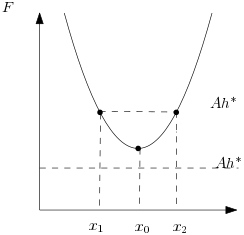
\includegraphics[width=5cm]{fig14.png} 
\end{figure}  
\begin{enumerate}
\item $h^* = \frac{F(x_0)}{A} \Rightarrow x = x_0,\;\; \Theta = \arccos x_0 = const$
\begin{figure}[H]
  \centering
  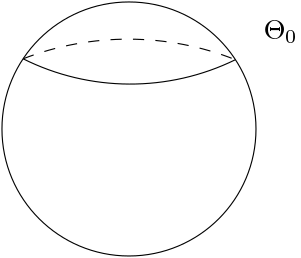
\includegraphics[width=4cm]{fig15.png} 
\end{figure}
\item $h^* > \frac{F(x_0)}{A}$: $\Theta_{min} = \arccos x_2$,~~ $\Theta_{max} = \arccos x_1$
\begin{figure}[h]
  \centering
  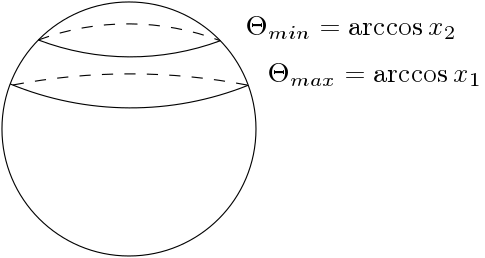
\includegraphics[width=6cm]{fig16.png} 
\end{figure}
\end{enumerate}

\begin{flalign*}
& \dot \psi = \frac{Cr_0x - k}{A(1 - x^2)} = 0 \Leftrightarrow x = x_* = \frac{k}{Cr_0} &\\
& F'_*(x_*) = 2Amgl > 0 &\\
\end{flalign*}

\begin{figure}[h]
  \centering
  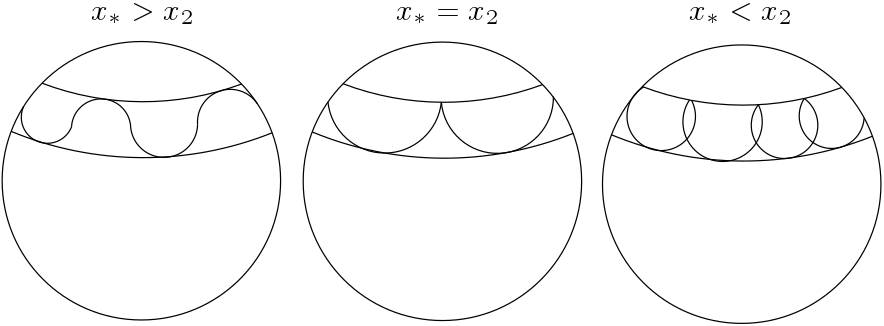
\includegraphics[width=14cm]{fig17.png} 
\end{figure}


\begin{ntc}
Если угловая скорость собственного вращения много больше скорости прецессии, т.е. $\dot \varphi \gg \dot \psi$, тело совершает псевдорегулярную пресессию.
\end{ntc}

\paragraph{Основные теоремы динамики}
\begin{flalign*}
& \v p = m \v v_s &\\
& \v k_O = [\v r_s, m \v v_s] + J_s \v \omega &\\
& T = \frac{1}{2}mv_s^2 + \frac{1}{2}(J_s\v \omega, \v \omega) &\\
\end{flalign*}

\begin{flalign*}
& \dot{\v p} = \sum\limits_{i = 1}^N F_i^{(e)}= \v F &\\
& \dot{\v k_O} = \sum p\v r_i, \v F_i^{(e)} = \v M_O &\\
& \dot T = \sum (\v F_i^{(e)}, \v v_i) &\\
\end{flalign*}

\begin{ntc}
\[
	\sum(\v F_i^{(e)}, \v v_i) = \dot T = (m \v w_s, \v v_s) + (\dot{(J_s\v\omega)}, \v \omega) = (\v F, \v v_s) + (\v M_s, \v \omega)
\]
\end{ntc}

\begin{ass}
Мощность внешних сил, действующих на твердое тело определяется равенством
\[
	\sum(\v F_i^{(e)}, \v v_i) = (\v p, \v v_p) + (\v M_p, \v \omega),
\]
где $p$ --- произвольная точка тела.
\end{ass}
\begin{proof}
\begin{flalign*}
& \sum (\v F_i^{(e)}, \v v_i) = \sum (\v F_i^{(e)}, \v v_p + [\v \omega, \rho_i]) = \left(\sum \v F_i^{(e)}, \v v_p\right) + (\v \omega, \sum [\v \rho_i, \v F_i]) = &\\
& = (\v p, \v v_p) + (\v M_p, \v \omega) &\\
\end{flalign*}
\end{proof}

\begin{df}
Две системы сил (в совокупности с точками их приложения), действующих на твердое тело называются эквивалентными, если они вызывают одно и то же движение тела.
\[
	\{ \v F_i, p_i \} \sim \{\v F_i', p_i'\}
\]
\end{df}
\begin{cor}
\[
	\{ \v F_i, p_i \} \sim {\v F_i', p_i'} \Leftrightarrow 
	\begin{cases}
	\sum \v F_i = \sum \v F_i' \\
	\sum [\v{OP}, \v F_i] = \sum [\v{OP}', \v F_i'] \\
	\end{cases}
\]	
\end{cor}
\begin{cor}
\[
	\{\v F_i, p_i\} \sim \{\v F, \v M_O, O\}, \quad \v F = \sum \v F_i,\;\; \v M_O = \sum [\v{OP}, \v F_i]
\]
\end{cor}
\begin{df}
$\v R$ --- равнодействующая системы сил $\{ \v F_i, \v p_i \}$, если существует точка $O$ тела, такая что $\{ \v F, p_i \} \sim \{\v R, O\}$
\end{df}
\begin{xmp}
Для двух сил, приложенных к разным концам твердого стержня в противоположном направлении, равнодействующая не существует.
\end{xmp}
\begin{xmp}
\[
	\{ m_i\v g, P_i \} \sim \{ m \v g, S \}
\]
\begin{flalign*}
& \sum m_i \v \rho = \left(\sum m_i\right)\v g = m\v g &\\
& \sum [\v {OP}, m_i \v g] = \sum [m_i \v {OP}, \v g] = \left[\sum m_i \v{OP}, \v g\right] = [m \v r_s, \v g] = [\v r_s, m\v g] &\\
\end{flalign*}
\end{xmp}

\[
	\v M_{O'} = \v M_O + [\v F, \v{OO'}]
\]

\begin{teo}
Если главный вектор внешних сил, действующих на твердое тело отличен от нуля, то существует такая точка, при приведении к которой, главный вектор и главный момент параллельны.
\[
	\v F \neq 0 \quad \exists A: \v M_A \parallel \v F
\]
\end{teo}
\begin{proof}
\begin{flalign*}
& \v M_a = \v M_O + [\v F, \v{OA}] = \lambda \v F \quad \big| \times \v F &\\
& [\v F, \v M_O] + \v F(\v F, \v{OA}) - F^2\v{OA} = 0 &\\
& \v{OA} = \frac{1}{F^2} [\v F, \v M_O] + \alpha \v F, \quad \forall \alpha = const
\end{flalign*}
\end{proof}
\begin{df}
Прямая, определяемая последним равенством называется осью динамического винта (осью минимальных моментов).
\end{df}
\begin{df}
$\lambda$ --- параметр винта.
\[
\lambda \v F = \v M_O + \left[ \v F, \frac{1}{F^2}[\v F, \v M_O] + \alpha \ F \right] = \v M_O + \frac{1}{F^2}\left( \v F(\v F, \v M_O) - F^2 \v M_O \right) = \frac{(\v F, \v M_O)}{F^2} \v F
\]
\[
	\lambda = \frac{(\v F, \v M_O)}{F^2}
\]
\begin{enumerate}
\item $\v F = 0: \quad \{ \v F_i, P_i\} \sim \{ \v M_O, O \}$
\item $\v F \neq 0, \lambda = 0: \{ \v F_i, P_i \} \sim \{\v R, A\}$
\item $\v F \neq 0, \lambda \neq 0: \{ \v F, P_i \} \sim \{\v F, \v M_A, A\}$
\end{enumerate}
\end{df}
  \lline{29.11.2017}\section{Уравнения Лагранжа}
$\v r_1, \ldots, \v r_N \in \R^3$

\begin{df}
Механическими связями называются ограничения на положения и скорости материальных точек системы, которые выполняются при всех действующих на систему силах.
\[
	\v r = (x_1, y_1, z_1, \ldots, x_N, y_N, z_N)^T \in \R^{3N}
\]
\begin{equation}
\label{29star}
f_j(\v r, \dot {\v r}, t) = 0, \quad j = 1, \ldots, k \text{ --- уравнение связи.}
\end{equation}
\end{df}

\subsection{Классификация связей}
\begin{enumerate}
\item \eqref{29star} --- двусторонная связь.
\item $\frac{\partial f_\alpha}{\partial t} = 0$ --- стационарная связь (склерономная).\\
$\frac{\partial f_\alpha}{\partial t} \neq 0$ --- нестационарная связь (реономная.)
\item $f_\alpha(\v r, t) = 0$ --- геометрическая.
\item $f_\alpha(\v r, \dot{\v r}, t) = 0$ --- дифференциальная связь.
\end{enumerate}

\subsubsection{Геометрические связи}
\begin{df}
$\Sigma = \{\v r : f_j(\v r, t) = 0, j = 1, \ldots, k \}$ --- пространство положений (конфигурационное пространство).
\end{df} 
\begin{df}
$n = dim \Sigma$ --- количество степеней свободы.
\end{df}
\begin{df}
$\v q = (q_1, \ldots, q_n)^T$ --- обобщенные локольные координаты.
\end{df}
$n = 3N - k$, где $k$ --- число уравнений связи, если \begin{enumerate}
\item функции связей гладкие ($\grad_{\v r} f_j \neq 0, \forall i \in 1, \ldots, k$)
\item $f_j$ --- независимые. ($\rank \left(\frac{\partial \v f}{\partial \v r}\right) = k$)
\end{enumerate}
\begin{df}
Функции $f_1, \ldots, f_n$ функционально независимы, если $F(f_1, \ldots, f_n) = 0 \Leftrightarrow F \equiv 0$
\end{df}
\begin{xmp}[Независимые функции]
$f_1(x) = x, f_2(x) = x^2, f_2 = f_1^2, F_2 = f_2 - f_1^2$.
\end{xmp}
\begin{xmp}
\begin{flalign*}
& f(\v r) = x^2 + y^2 + z^2 = 0 \Leftrightarrow x = y = z = 0 &\\
& \grad f |_{x = 0} = 0 \qquad n = 0 \neq 3\cdot 1 - 1 = 2 &\\
\end{flalign*}

\end{xmp}
\begin{xmp}
\begin{flalign*}
& |\v r_i - \v r_j| = c_{ij} = const &\\
& k = \frac{N(N - 1)}{2} \qquad n = 6 \neq 3N - \frac{N(N - 1)}{2}, \quad N > 4
\end{flalign*}
\end{xmp}

$\v r = \v r(\v q, t)$
\begin{xmp}
\begin{flalign*}
& \v v_k = 0, n = 2, \v q = (x, \v \varphi)^T &\\
& \v v_k = \v v_0 + [\v \omega, \v{OK}] = \dot x, \v e_x + [- \dot \varphi \v e_z, - R \v e_y] = (\dot x - R \dot \varphi)\v e_x = 0 \Leftrightarrow &\\
& \Leftrightarrow \dot x - R \dot \varphi = 0 &\\
& \int d x = \int R d\varphi &\\
& x - x_0 = R(\varphi - \varphi_0) &\\
\end{flalign*}
\end{xmp}
\begin{ntc}
\[
	f(\v r, t) \equiv 0 \Leftrightarrow \frac{\partial f}{\partial \v r}\dot{\v r} + \frac{\partial f}{\partial t}
\]
\end{ntc}
\begin{df}
Дифференциальная связь называется голономной (интегрируемой), если она может быть представлена в эквивалентной геометрической форме. В противном случае связь неголономна (неинтегрируема).
\end{df}
\begin{xmp}[конек Чаплыгина]
\begin{flalign*}
&\v v_k \parallel \v l, \quad n = 3, \v q = (x, y, \varphi)^T &\\
& \v v_k = \dot x\v e_x + \dot y \v e_y \parallel \cos \varphi \v e_x + \sin \varphi \v e_y &\\
& \frac{\dot y}{\dot x} = \tg \varphi \Rightarrow \dot y = \dot x \tg \varphi &\\
& \text{Пусть } \exists f(x, y, \varphi, t) = 0 \Leftrightarrow \dot y = \dot x \tg \varphi &\\
& \frac{\partial f}{\partial x}\dot x + \frac{\partial f}{\partial y}\dot y + \frac{\partial f}{\partial \varphi}\dot \varphi + \frac{\partial f}{\partial t} \Leftrightarrow \dot y = \dot x \tg \varphi &\\
& \dot x\left( \pd{f}{x} + \pd{f}{y} \tg \varphi \right) + \pd{f}{\varphi} \dot \varphi + \pd{f}{t} = 0 \Leftrightarrow &\\
& \Leftrightarrow \begin{cases}
\pd{f}{t} = 0 \\
\pd{f}{\varphi} = 0 \\
\pd{f}{x} + \pd{f}{y} \tg \varphi = 0 \Leftrightarrow \pd{f}{x} = \pd{f}{y} = 0 \\
\end{cases}
\Leftrightarrow f = 0 &\\
\end{flalign*}
\end{xmp}
\begin{flalign*}
& \v a(\v r)\dot{ \v r} + b(\v r) = 0 \text{ --- интегрируема, если } &\\
& \exists f: \pd{f}{\v r} = \v a, \pd{f}{t} = b \Leftrightarrow \Phi = 
\left(
\begin{matrix}
\pd{a_1}{q_1} & \ldots & \pd{a_1}{q_n} & \pd{a_1}{t} \\
\vdots & \ddots & \vdots & \vdots \\
\pd{a_n}{q_1} & \ldots & \pd{a_n}{q_n} & \pd{a_n}{t} \\
\end{matrix}
\right) &\\
\end{flalign*}
Критерий ($n = 3$) $a_1\dot q_1 + a_2\dot q_2 + a_3\dot q_3 = 0$ --- интегрируемая $\Leftrightarrow \v a \rot \v a = 0$

\subsection{Действительные и виртуальные перемещения}
\begin{flalign*}
& \v r = \v r(\v q, t) &\\
& \v v = \dot{\v r} = \frac{d \v r}{d t} = \pd{\v r}{\v q} \dot{\v q} + \pd{\v r}{t} &\\
& d \v r = \pd{\v r}{\v q} d \v q + \pd{\v r}{t}dt \text{ --- действительные перемещения.} &\\
& \Sigma = \{ \v r, f_j(\v r) = 0, j = 1, \ldots, k \} &\\
& \sum_{i = 1}^n \pd{f_j}{\v r_i}d\v r_i + \pd{f_j}{t}dt = \pd{f_j}{\v r}d\v r + \pd{f_j}{t}dt = 0 &\\
& \delta \v r = \sum_{i = 1}^N \pd{\v r}{q_i}\delta q_i \text{ --- виртуальные перемещения.} &\\
& \pd{f_j}{\v r} \delta \v r = 0, \quad j = 1, \ldots, k &\\
\end{flalign*}
\begin{ntc}
Если связи стационарные, то пространство действительных и виртуальных перемещений совпадают\footnote{Написано неразборчиво, доверять этому утверждению не стоит.}.
\end{ntc}

\subsection{Идеальные связи и общие уравнения динамики. Принцип освобождаемости связи. (Уравнения Лагранжа первого рода)}
Если к активным силам, действующим на механическую систему, добавляются силы, с помощью которых реализуется уравнения связи, то систему можно рассматривать как свободную.

$\v R_i$ --- сила реакции, действующая на $m_i$
\[
	m_i \ddot{\v r_i} = \v R_i + \v F_i
\]
\begin{df}
Связи идеальные, если при любом виртуальном перемещении системы выполняется равенство
\[
	\sum_{i = 1}^n (\v R_i, \delta \v r_i) = 0
\]
\end{df}

\begin{flalign*}
& \v R_i = m_i \ddot{\v r_i} - \v F_i &\\
& \sum_{i = 1}^N (m_i \ddot{\v r_i}, \delta \v r_i) = 0 &\\
\end{flalign*}

\subsubsection{Принцип Даламбера-Лагранжа\protect\footnote{Также принцип виртуальных перемещений.}}
\begin{ass}
Если связи, наложенные на мезаническую систему идеальные, то при любом ее движении и любом виртуальном перемещении выполнено равенство
\begin{equation}
	\label{29sstar}
	\sum_{i = 1}^N(m_i \ddot{\v r_i} - \v F_i, \delta \v r_i) = 0
\end{equation}
\end{ass}
\begin{ass}[Обратное]
Если связи идеальные и какое-то движение удовлетворяет \eqref{29sstar}, то это движение является действительным движением системы.
\end{ass}
\begin{proof}
$\Rightarrow$\\
Если связи идеальны, то
\begin{flalign*}
& \v r = \v r(t) \Leftrightarrow \sum_{i = 1}^N(m_i \ddot{\v r_i} - \v F_i, \delta \v r_i) = 0 &\\
& \ddot{\v r_i} = \ddot{\v r_i}(\v r_1, \ldots, \v r_N, \dot{\v r}_N, \ldots, \dot{\v r}_N, t) &\\
& M = \diag(m_1, m_1, m_1, m_2, m_2, m_2, \ldots, m_N, m_N, m_N) &\\
& \v R = (R_{1x}, R_{1y}, R_{1z}, \ldots, R_{Nx}, R_{Ny}, R_{Nz})^T &\\
& \v F = (F_{1x}, F_{1y}, F_{1z}, \ldots, F_{Nx}, F_{Ny}, F_{Nz})^T &\\
& \eqref{29sstar} \Leftrightarrow (M \ddot{\v r} - \v F, \delta \v r) = 0, \v R = M\ddot{\v r} - \v F &\\
& \delta \v r = \pd{f}{\v r} &\\
& \ddot{\v r} = \ddot{\v r}(\ddot{\v r}, \dot{\v r}, t) \Rightarrow \v R = \v R(\v r, \dot{\v r}, t) &\\
\end{flalign*}
% \end{proof}
  \lline{06.12.2017}% \section{Coming soon}
\begin{center}
\line(1,0){250}
\end{center}
Вроде бы это еще не в другую сторону, но уже и не в ту (Тут был перерыв между лекциями)
\begin{flalign*}
& \v r = (x_1, \ldots, z_N)^T \in \mathbb{R}^{3N} &\\
& \v F = (F_{1x}, \ldots, F_{Nz})^T \in \mathbb{R}^{3N} &\\
& f_I = (\v , t) = 0, i = \overline{1,\ldots k} &\\
& \v \varphi_i \grad_{\v r} \rho_i \in \mathbb{R}^{3N} &\\
& \Phi = \left( \begin{matrix}
\frac{\partial f_1}{\partial x_1} & \ldots & \frac{\partial f_1}{\partial z_N} \\
\vdots & \ddots & \vdots \\
\frac{\partial f_k}{\partial x_1} & \ldots & \frac{\partial f_k}{\partial z_N} \\
\end{matrix} \right) &\\
& \rank{\Phi} = k &\\
\end{flalign*}
Число степеней свободы --- размерность пространства виртуальных перемещений.
$\delta \v r: \left( \pd{f_i}{\v r}, \delta \v r \right) = (\v \varphi_i, \delta \v r) = 0, \quad \forall i = 1, \ldots, k \Leftrightarrow \Phi d\v r = 0, \underline{n = 3N - k}$\\
$\v R \in \R^{3N}$ --- реакции $(\v R, \delta \v r) = 0$ --- условия идеальной связи.
\begin{center}
\line(1,0){250}
\end{center}
% \begin{teo}
% Принцип Даламбера-Лагранжа: если связи идеальные, то
% \[
% 	\v r(t) \Leftrightarrow (M\ddot{\v r} - \v F, \delta \v r) = 0
% \]
% \end{teo}
% \begin{proof}
% $\Rightarrow \ldots$\\
$\Leftarrow$
\begin{flalign*}
& I &\\
& (M \ddot{\v r} - \v F, \delta \v r) = 0 \xrightarrow{?} \ddot{\v r} = \ddot{\v r}(\v r, \dot{\v r}, t) &\\
& (\v \varphi_i, \delta \v r) = 0 \quad \forall i = \overline{1, \ldots k} \Rightarrow &\\
& \Rightarrow \delta \v r \perp \pi = \{ c_1\v \varphi_1 + c_2 \v \varphi_2 + \ldots + c_k \v \varphi_k,~~ c_i \in \mathbb{R},~~ i \in \overline{1, \ldots k} \} &\\
&(M \ddot{\v r} - \v F, \delta r) = 0 \Rightarrow M\ddot{\v r} - \v F \in \pi \rightarrow &\\
& \Rightarrow \exists \lambda_1, \ldots, \lambda_k: M\ddot{\v r} - \v F = \lambda_1 \v \varphi_1 + \ldots + \lambda_k \v \varphi_k = \Phi^T \v \lambda &\\
& \v \lambda = (\lambda_1, \ldots, \lambda_k)^T \in \mathbb{R}^k \rightarrow \ddot{\v r} = M^{-1}\overline{F} + M^{-1}\Phi^T \v \lambda &\\
\end{flalign*}
\begin{flalign*}
& II &\\
& f_i(\v r, t) \equiv 0 &\\
& \frac{d f_i}{d t} = \left( \underbrace{\frac{\partial f_i}{\partial \v r}}_{\v \varphi_i},~~ \dot{\v r} \right) + \frac{\partial f_i}{\partial t} = 0, \quad \forall i = \overline{1, \ldots k} &\\
& \Phi \dot{\v r} + \v \beta(\v r, t) = 0 &\\
& \Phi \dot{\v r} + \psi(\v r, \dot{\v r}, t) = 0 \Rightarrow &\\
& \Phi M^{-1} \v F + \Phi M^{-1} \Phi^T \v \lambda + \v \psi = 0 \Rightarrow &\\
& \Rightarrow \Phi M^{-1} \Phi^T \v \lambda = \v h(\v r, \dot{\v r}, t) &\\
\end{flalign*}
\begin{flalign*}
III &\\
\forall \v u \neq 0: & (\Phi M^{-1} \Phi^T\v u, \v u) = (M^{-1} \Phi^T \v u, \Phi^T \v u) = &\\
& = (M^{-1}\v x, \v x) > 0, \text{т.к.} &\\
& a) det M^{-1} = (det M)^{-1} \neq 0, &\\
& b) \v x = \Phi^T \v u \neq 0, \quad \forall \v u \neq 0. &\\
& \Rightarrow det(\Phi M^{-1} \Phi^T) \neq 0 \Rightarrow \v \lambda = (\Phi M^{-1} \Phi^T)^{-1} h(\v r, \dot {\v r}, t) = \lambda(\v r, \dot{\v r}, t) \Rightarrow &\\
& \v R = M \ddot{\v r} - \v F = \v R(\v r, \dot{\v r}, t) &\\
\end{flalign*}
\end{proof}

\begin{ntc}
Принцип виртуальных перемещений справедлив и для неголономных систем и доказывается аналогично.
\end{ntc}

\begin{ntc}
\[
	\begin{cases}
	M\ddot{\v r} - \v F = \Phi^T \v \lambda \\
	R_i(\v r, t) = 0, i = 1, \ldots, k \\
	\end{cases}
	\text{ --- уравнения Лагранжа 1 рода (Это неточно)}
\]
\end{ntc}

\subsection{Обобщенные силы}
\begin{flalign*}
& \v r = \v r(\v q, t), \quad (\v u = \v r_i(\v q, t)), \v q = (q_1, \ldots, q_n)^T &\\
& \delta A = \sum\limits_{i = 1}^N (\v F_i, \delta \v r_i) = (\v F, \delta \v r) = \left( \v F, \sum\limits_{j = 1}^N \frac{\partial \v r}{\partial q_j} \delta q_j \right) = \sum\limits_{j = 1}^{N}\left( \v F, \frac{\partial \v r}{\partial q_j} \right)\delta q_i = \sum_{j = 1}^n Q_j\delta q_j = (\v Q, \delta \v q)
\end{flalign*}

\begin{df}
\[
	Q_j = (\v F, \frac{\partial \v r}{\partial q_j}) = \sum\limits_{i = 1}^{N}(\v F_i, \delta \v r_i)
\]
--- обобщенная сила, соответствующая координате $q_j$.
\end{df}

\begin{ass}
Если координата $q_l$ --- декартова координата центра масс всей системы, то соответствующая ей обобщенная сила равна проекции главного вектора внешних сил системы на соответствующую декартову ось.
\[
	q_l = x_s \Rightarrow Q_l = (\v F, \v e_x)
\]
\end{ass}
\begin{proof}
\begin{flalign*}
& \delta q_j = 0, \quad j \neq l \Rightarrow \delta \v r_i = \delta x_s \v e_x &\\
& \delta A = \sum\limits_{i = 1}^{N}(\v F_i, \delta \v r_i) = \sum\limits_{i = 1}^{N}(\v F_i, \delta x_S\v e_x) = \left(\sum\limits_{i = 1}^{N}\v F_i, \v e_x\right) \delta x_s = Q_l \delta q_l &\\
\end{flalign*}
\end{proof}

\begin{xmp}[АТТ]
\begin{flalign*}
& \v r_i = \v r_p + \v \rho_i = \v r_p + \sum\limits_{\alpha = 1}^3 \rho_{i\alpha} \v e_\alpha, &\\
& \{ \v e_1, \v e_2, \v e_3 \} \text{ --- базис, связянный с телом.} &\\
& \v r_i = \v r_i(\v q, t), \quad \v r_p = \v r_p(\v q, t), \quad \v e_\alpha = \v e_\alpha (\v q, t) &\\
& \rho_{i\alpha} = const &\\
& \left( \dot{\v e_\alpha} = \sum\limits_{j = 1}^N \frac{\partial \v e_\alpha}{\partial q_j}\dot q_j + \frac{\partial \v e_\alpha}{\partial t} \Rightarrow \frac{\partial \dot{\v e}_\alpha}{\partial \dot q_j} = \frac{\partial \v e_\alpha}{\partial q_j} \right) &\\
& \delta e_\alpha = \sum_{j = 1}^N\pd{\v e_\alpha}{q_j}\delta q_j = \sum \pd{\dot{\v e_\alpha}}{\dot q_j} \delta q_j = \sum_{j = 1}^N \pdd{[\v \omega, \v e_\alpha]}{\dot q_j} \delta q_j = \sum_{j = 1}^N \left[\pd{\v \omega}{\dot q_j}, \v e_\alpha\right]\delta q_j &\\
& \delta \v u = \delta \v r_p + \sum\limits_{\alpha = 1}^3 \rho_{i\alpha} \sum \left[ \frac{\partial \v \omega}{\partial \dot q_j}, \v e_\alpha \right] \delta q_i = &\\
& = \delta \v r_p + \sum\limits_{j = 1}^N\left[ \frac{\partial \v \omega}{\partial \dot q_j}\delta q_j, \sum\limits_{\alpha = 1}^3 \rho_{i\alpha} \v e_\alpha \right] = &\\
& = \delta \v r_p + \left[ \sum\limits_{j = 1}^N \pd{\v \omega}{\dot q_j}\delta q_j, \v \rho_j \right] = \delta \v r_p + [\v \omega_\delta, \v \rho_i], \quad \v \omega_\delta = \sum_{j = 1}^n \pd{\v \omega}{\dot q_j} \delta q_j
\end{flalign*}
\begin{flalign*}
& \delta A = \sum_{i = 1}^N(\v F_i, \delta \v r_i) = \sum_{i = 1}^N(\v F_i, \delta \v r_p) + \sum_{i = 1}^N(\v F_i, [\v \omega_\delta, \v \rho]) = &\\
& = (\sum \v F_i, \delta r_p) + \left(\v \omega_\delta, \sum_{i = 1}^N[\v \rho_i, \v F_i]\right) = (\v F, \delta \v r_p) + (\v \omega_\delta, \v M_p) &\\
\end{flalign*}
\end{xmp}

\begin{cor}
$\v F^{(i)} = 0$, $\v M_p^{(i)} = 0 \Rightarrow$ внутренние связи в твердом теле идеальны.
\end{cor}
\begin{xmp}[АТТ с неподвижной точкой]
\begin{flalign*}
& n = 3, &\\
& q = (\varphi, \psi, \Theta)^T, \quad \v \omega = \dot \psi \v e_z + \Theta \v e_{x_1} + \dot \varphi \v e_\zeta &\\
& \v \omega \delta = \delta \psi \v e_z + \delta \Theta \v e_{x_1} + \delta \varphi \v e_\zeta &\\
& \delta A = \left( \v M_O, \delta \psi \v e_z + \delta \Theta \v e_x + \delta \varphi \v e_\zeta \right) = &\\
& = (\v M_O, \v e_z)\delta \psi + (\v M_O, \v e_{x_1})\delta \Theta + (\v M_O, \v e_\zeta)\delta \varphi
\end{flalign*}
\end{xmp}

\begin{ass}
Если обобщенная координата --- это угол поворота силы относительно некоторой оси, то обобщенная сила --- это момент силы относительно этой же оси.
\end{ass}

\subsection{Уравнения Лагранжа второго рода}
\begin{teo}
Если связи, наложенные на механическую систему, идеальны и голономны, то уравнения ее движения имеют вид
\[
	\frac{d}{dt}\frac{\partial T}{\partial \dot{\v q}} - \frac{\partial T}{\partial \v q} = \v Q
\]
\end{teo}
\begin{proof}
\begin{flalign*}
& \sum\limits_{i = 1}^N (M_i \ddot{\v r}_i - \v F_i, \delta \v r_i) = 0, \quad \v r_i = \v r_i(\v q, t) &\\
& \sum\limits_{i = 1}^N (m_i \ddot{\v r}_i - \v F_i, \sum\limits_{j = 1}^n \frac{\partial \v r_i}{\partial q_j}\delta q_j) = 0 &\\
& \sum\limits_{j = 1}^n \left( \sum\limits{i = 1}^N(m_i \ddot{ \v r_i} - \v F_i. \frac{\partial \v r_i}{\partial q_j}) \right)\delta q_j = 0 &\\
& \delta q_1, \ldots, \delta q_n \text{ --- независимые} \Rightarrow &\\
& \Rightarrow \sum\limits_{i = 1}^N \left( m_i \ddot{\v r_i} - F_i, \frac{\partial \v r_i}{\partial q_j} \right) = 0, \quad \forall j = \overline {1,\ldots n} &\\
& \sum\limits_{i = 1}^N \left( m_i \ddot{\v r_i}, \frac{\partial \v r_i}{\partial q_j} \right) = \underbrace{\sum \limits_{i = 1}^N \left( \v F_i, \frac{\partial \v r_i}{\partial q_j} \right)}_{Q_j} &\\
& \sum_{i = 1}^N\left( m_i, \ddot{\v r_i}, \pd{\v r_i}{\dot q_j} \right) = \frac{d}{dt}\left( \sum_{i = 1}^N \left( m_i \dot{\v r_i}, \pd{\v r_i}{q_j} \right) \right) - \sum_{i = 1}^N \left(m_i \dot{\v r_i}, \frac{d}{dt}\pd{\v r_i}{q_j}\right) = &\\
& = \frac{d}{dt}\left( \sum_{i = 1}^N m_i\dot {\v r_i}, \pd{\dot {\v r_i}}{\dot q} \right) - \sum_{i = 1}^N\left(m_i\dot{\v r}, \pd{\dot{\v r_i}}{q_i}\right) = &\\
& = \frac{d}{dt}\pdd{\sum_{i = 1}^N m_i \frac{(\dot{\v r_i}, \dot{\v r_i})}{2}}{\dot q_j} - \pdd{\sum_{i = 1}^N m_i\frac{(\dot {\v r_i}, \dot {\v r_i})}{2}}{q_j} = \frac{d}{dt}\pd{T}{\dot q_j} - \pd{T}{q_j} &\\
\end{flalign*}
\end{proof}

\begin{cor}
Связи идеальны и голономны, а силы потенциальны $\Rightarrow$
\[
	\frac{d}{dt} \frac{\partial L}{\partial \dot{\v q}} - \frac{\partial L}{\partial \v q} = 0, L = T - \Pi
\]
\end{cor}
\begin{df}
$L$ --- лагранжиан системы, система лагранжева.
\end{df}
\begin{flalign*}
& \exists \Pi(\v r_1, \ldots, \v r_N, t), \quad \grad_{\v r_i} \Pi = -\v F_i &\\
& \delta A = \sum_{i = 1}^N(\v F_i, \delta \v r_i) = (\v F, \delta \v r) = - \left( \pd{\Pi}{\v r}, \delta \v r \right) = &\\
& = - \sum_{j = 1}^N \left( \pd{\Pi(\v r(\v q, t), t)}{\v r}, \pd{\v r}{\v q_j} \right) \delta q_j = -\sum_{j = 1}^N \pd{\Pi}{q_j}\delta q_j \Rightarrow &\\
& \Rightarrow Q_j = - \pd{\Pi}{q_j} &\\
& L = T - \Pi = T(\v q, \dot{\v q}, t) - \Pi(\v q, t) &\\
& \pd{L}{\v q} = \pd{T}{\v q} - \pd{\Pi}{\v q} = \pd{T}{\v q} + \v Q
\end{flalign*}
  \lline{13.12.2017}\begin{flalign*}
& \v q = (q_1, \ldots, q_n)^T, \quad \dot{\v q} =  (\dot q_1, \ldots, \dot q_n), \quad \v r_i = r_i(\v q, t) &\\
& T = \frac{1}{2} \sum_{i = 1}^N m_i \dot{\v r_i}^2 =  \underbrace{\frac{1}{2}\sum_{i = 1}^N m_i \left( \sum_{j = 1}^N \pd{\v r_i}{q_j} + \pd{\v r_i}{t} \right)^2}_{\text{структура кинетической энергии}} = T_2 + T_1 + T_0 &\\
& T_0 = \frac{1}{2} \sum_i \left( \pd{\v r_i}{t} \right)^2 &\\
& T_1 = \sum_j \underbrace{\sum_i m_i \left( \pd{\v r_i}{\v q_j}, \pd{\v r_i}{t} \right)}_{b_j} \dot q_j = \sum_j b_j\dot q_j = (\v b, \dot{\v q}) &\\
& \v b = (b_1, \ldots, b_n)^T, \v b = \v b(\v q, t) &\\
& T_2 = \frac{1}{2} \sum_{j, k} \underbrace{\sum_i m_i \left( \pd{\v r_i}{q_k}, \pd{\v r_i}{q_j} \right)}_{a_{jk}} \dot q_j \dot q_k = \frac{1}{2}(A\dot {\v q}, \dot{\v q}), \quad A = (a_{jk}), A = A^T
\end{flalign*}
\begin{ass}
$A$ --- положительно определенная матрица.
\end{ass}
\begin{proof}
\begin{flalign*}
& \delta \v q = (\delta q_1, \ldots, \delta q_n)^T, \delta \v r = \sum_{j = 1}^n \pd{\v r}{q_j} \delta q_j &\\
& \delta \v r = 0 \Leftrightarrow \delta \v q = 0 &\\
& (A\delta \v q, \delta \v q) = \sum_{j = 1}^N m_i \sum_{j = 1}^n \left( \pd{\v r_i}{q_j}, \delta a_j \right)^2 = \sum_{i = 1}^N m_i(\delta r_i)^2 = (M\delta \v r, \delta \v r) > 0, \forall \delta \v q \neq 0 &\\
\end{flalign*}
\end{proof}
\begin{cor}
$\det A \neq 0$.
\end{cor}

\subsection{Свойства уравнений Лагранжа}
\paragraph*{Уравнения Лагранжа:}
\begin{enumerate}
\item Связи идеальны и голономны:
\[
	\frac{d}{dt}\pd{T}{\dot{\v q}} - \pd{T}{\v q} = \v Q
\]
\item Связи идеальны и голономны, а активные силы потенциальны:
\[
	\frac{d}{dt}\pd{L}{\dot{\v q}} - \pd{L}{\v q} = 0
\]
\item Связи идеальны и голономны, а активные силы не потенциальны:
\[
	\frac{d}{dt}\pd{L}{\dot{\v q}} - \pd{L}{\v q} = \v Q^*
\]
\end{enumerate}
Где $L = T - \Pi, \quad \v Q^*$ --- обобщенные силы, вызванные непотенциальными активными силами.\\
$\v Q^*(\v q, \dot{\v q}, t)$ --- обобщенный потенциал, если $\exists V(\v q, \dot{\v q}, t)$.
\[
	\frac{d}{dt}\pd{V}{\dot{\v q}} - \pd{V}{\v q} = \v Q^*  \Rightarrow L = T - \Pi - V
\]
\[
	\frac{d}{dt}\pd{L}{\v q} - \pd{L}{\v q} = 0
\]
\begin{enumerate}
\item Ковариантность по отношению к выбору обобщенных координат
\[
	\v q \longrightarrow T(\v q, \dot{\v q}, t),\quad \v Q (\v q, \dot{\v q}, t) \longrightarrow \frac{d}{dt}\pd{T}{\dot{\v q}} - \pd{T}{\v q} = \v Q
\]
\[
	\v q' \longrightarrow  T'(\v q', \dot{\v q}, t) = T(\v q, (\v q', t),\; \dot {\v q'}(\dot{\v q'}, \v q', t),\; t),\quad  \v Q'
\]
\item Калибровочная инвариантность
\begin{ass}
Уравнения Лагранжа не меняются при добавлении кинетической энергии полной производной гладкой функции от обобщенных координат и времени.
\[
	T' = T + \frac{d}{dt}f(\v q, t)
\]
\end{ass}
\begin{proof}
\begin{flalign*}
& \frac{d}{dt}f(\v q, t) = \sum_{i = 1}^n \pd{f}{q_i} \dot q_i + \pd{f}{t} &\\
& \pd{\dot f}{\dot q_i} = \pd{f}{q_i} \qquad \frac{d}{dt} \pd{\dot f}{\dot q_i} = \sum_{k = 1} \pd{^2 f}{q_k \partial q_i} \dot q_k + \pd{^2 f}{t \partial q_i} = \sum_{k = 1}^n \pd{^2 f}{q_i \partial q_k} \dot q_k + \pd{^2 f}{q_i \partial t} = \pd{\dot f}{q_i} \Rightarrow &\\
& \Rightarrow \frac{d}{dt}\pd{\dot f}{\dot{\v q}} - \pd{\dot f}{\v q} = 0 \Rightarrow \frac{d}{dt}\pd{T'}{\dot{\v q}} - \pd{T'}{\v q} = \frac{d}{dt}\pd{T}{\dot{\v q}} - \pd{T}{\v q} = \v Q
\end{flalign*}
\end{proof}
\begin{ass}
В Лагранжевой системе
\[
	L' = c_1 L + \dot f + c_2, \quad c_1 \neq 0, \quad c_1 = const, c_2 = const
\]
\end{ass}
\item Разрешимо относительно $\ddot{ \v q}$
\begin{proof}
\begin{flalign*}
& \pdd{A \dot{\v q}, \dot{\v q}}{\dot q_i} = \pdd{\sum_{j, k}q_{jk}\dot q_j \dot q_k}{\dot q_i} = &\\
& = \sum_k a_{ik} \dot q_k + \sum_j a_{ji}\dot q_j = 2\sum_k a_{ik}\dot q_k &\\
& \pdd{A \dot{\v q}, \dot{\v q}}{\dot{\v q}} = 2A\dot{\v q} &\\
& \left( \pd{T_2}{\dot{\v q}}, \dot{\v q} \right) = 2T_2\text{ (формально, теорема об однородных функциях)} &\\
& \frac{d}{dt}\pd{T}{\dot{\v q}} = \frac{d}{dt}\left( \frac{1}{2} (A \dot{\v q}, \dot{\v q}) + (\v b, \dot{\v q}) + T_0 \right) = \frac{d}{dt}\left( A(\v q, t) \dot{\v q} + \v b(\v q, t) \right) = &\\
& = A\ddot{\v q} + \v \beta(\v q, \dot{\v q}, t) &\\
& \pd{T}{\v q} = \pdd{T_2 + T_1 + T_0}{\v q} = \v \varphi(\v q, \dot{\v q}, t) &\\
& A \ddot{\v q} + \v \beta - \v \varphi = \v Q \Rightarrow A \ddot{\v q} = \v \psi(\v q, \dot{\v q}, t) &\\
\end{flalign*}
\begin{equation}
\label{lastone}
\det A \neq 0 \Rightarrow \ddot{\v q} = A^{-1} \v \psi(\v q, \dot{\v q}, t) = f(\v q, \dot{\v q, t})
\end{equation}
\end{proof}
\begin{ntc}
Система \eqref{lastone} может быть записана в форме Коши:
\[
	\begin{cases}
	\dot{\v q} = \v v \\
	\dot{\v v} = f(\v q, \dot{\v q}, t) \\
	\end{cases}
	\qquad
	\begin{matrix}
	& \v x = (q_1, \dots, q_k, v_1, \ldots, v_n)^T \in \R^{2n} \\
	& \dot{\v x} = \v F(\v x, t) \\
	\end{matrix}
\]
\end{ntc}
\end{enumerate}

\subsection{Первые интегралы Лагранжевой системы координат}
\[
	\frac{d}{dt}\pd{L}{\dot{\v q}} - \pd{L}{\v q}, \quad L = T - \Pi
\]
\subsubsection{Циклический интеграл}
\begin{df}
$q_1$ --- циклическая координата, если $\pd{L}{q_1} = 0$.
\end{df}
\begin{ass}
\[
	\pd{L}{q_1} = 0 \Rightarrow \pd{L}{\dot{\v q}} = c = const
\]
\end{ass}
\begin{proof}
\[
	\pd{L}{q_1} = 0 \Rightarrow \frac{d}{dt} \pd{L}{\dot q_1} = 0 \Rightarrow \pd{L}{\dot{\v q_1}}	= c = const
\]
\end{proof}
\begin{xmp}[Движение точки в центральном поле]
\begin{flalign*}
& L = T - \Pi = \frac{m}{2}\left( \dot r^2 + r^2 \dot\varphi^2 \right) - \Pi(r), \quad F = F(r) &\\
& \pd{L}{\varphi} = 0 \Rightarrow \pd{L}{\dot \varphi} = m r^2 \dot \varphi = c  = const
\end{flalign*}
\end{xmp}
\begin{xmp}
Волчок Лагранжа.
\end{xmp}

\subsubsection{Обобщенный интеграл (интеграл Пенлеве-Якоби)}
\begin{ass}
\[
	\pd{L}{t} = 0 \Rightarrow E = \left( \pd{L}{\v q}, \dot{\v q} \right) - L = const
\]
\end{ass}
\begin{proof}
\begin{flalign*}
& \pd{L}{t} = \left( \frac{d}{dt} \pd{L}{\dot{\v q}}, \dot{\v q} \right) + \left( \pd{L}{\dot{\v q}}, \dot{\v q} \right) - \left( \pd{L}{\dot{\v q}}, \dot{\v q} \right) - \pd{L}{t} = \left( \frac{d}{dt}\pd{L}{\dot{\v q}} - \pd{L}{\v q}, \dot{\v q} \right) - \pd{L}{t} = \pd{L}{t} &\\
& \pd{L}{t} = 0 \Rightarrow \frac{d}{dt}E = 0 \Rightarrow E = const &\\
\end{flalign*}
\end{proof}
\begin{ntc}
\begin{flalign*}
& L = T - \Pi = T_2 + T_1 + T_0 - \Pi &\\
& E = \left( \pd{L}{\dot {\v q}}, \v q \right) - L = \underbrace{\left( \pd{T_2}{\dot{\v q}}, \dot{\v q} \right)}_{2T_2} + \underbrace{\left( \pd{T_1}{\dot {\v q}, \dot{\v q}} \right)}_{T_1} + 0 - T_2 - T_1 - T_0 + \Pi = T_2 - T_0 + \Pi &\\
& \text{если } T = T_2 \text{, то } E = T_2 + \Pi = T + \Pi \text{ --- полная энергия} &\\
& \text{если } T \neq T_2 \text{, то } E = T_2 - T_0 + \Pi \text{ --- обобщенная энергия} &\\
\end{flalign*}
\end{ntc}

\begin{cor}
Если связи идеальные, голономные и стационарные, а активные силы консервативны, то
\[
	T + \Pi = const
\]
\end{cor}
\begin{proof}
\begin{enumerate}
\item Связи идеальные, голономные, значит силы потенциальны.
\item Связи стационарны $ \Rightarrow \v r_i(\v q, t) = \v r_i(q)$
\[
 	\pd{\v r}{t} = 0 \Rightarrow T_1 = 0, T_0 = 0, T = T_2.
\] 
\item
\[
	\pd{\Pi}{t} = 0 \Rightarrow \pd{L}{t} = 0
\]
\[
	\Rightarrow E = T_2 + \Pi - T + \Pi = const
\]
\end{enumerate}
\end{proof}

\paragraph*{Обобщение}
\begin{flalign*}
& \frac{d}{dt} \pd{L}{\dot{\v q}} - \pd{L}{\v q} = \v Q^*, L = T_2 - \Pi(\v q) &\\
& \frac{dE}{dt} = \left( \frac{d}{dt}\pd{L}{\dot{\v q}} - \pd{L}{\v q}, \dot{\v q} \right) + 0 = (Q^*, \dot{\v q})
\end{flalign*}
\begin{ntc}
\[
	(\v Q, \dot{\v q}) = \sum_j Q_j^*\dot q_j = \sum_{j = 1}^n\left( \sum_{i = 1}^N(\v F_i^*, \pd{\v r_i}{q_j}) \right)\dot q_j = \sum_{i = 1}^N\left( \v F_i^*, \sum \pd{\v r_i}{q_j}\dot q_j \right) = \sum_{i = 1}^N (\v F_i^*, \v v_i) \text{, т.к.} \pd{\v r_i}{t} = 0
\]
\end{ntc}
\begin{df}
$E = (\v Q^*, \dot{\v q}) \equiv 0  \quad \forall\dot{\v q}$ --- $\v Q^*$ --- гироскопическая
\end{df}
\begin{df}
$E = (\v Q^*, \dot{\v q}) \leqslant 0$ --- $\v Q^*$ --- диссипативная
\end{df}
\begin{df}
$E = (\v Q^*, \dot{\v q}) < 0 \forall \quad \dot{\v q} \neq 0$ --- $\v Q^*$ --- гироскопическая
\end{df}
\end{document}
